\documentclass[output=paper,hidelinks]{langscibook}
\ChapterDOI{10.5281/zenodo.13347658}
\author{Myriam Lapierre\affiliation{University of Washington}}
\title{Postoralized and devoiced nasals in Panãra (Jê): ND > NT}  
\abstract{This paper discusses a sound change from ND $>$ NT in Panãra. Postnasal devoicing in Panãra is categorical, and articulatory data suggests that vocal fold vibration is actively suppressed when the velum is maximally open. Panãra differs structurally from other languages for which a change from ND $>$ NT has been observed, as the NC segments in Panãra are monosegmental and arise from a synchronic process of postoralization and devoicing of nasal stops /N/. I argue that this case of ND $>$ NT is motivated by the need to increase the perceptual salience of the oral release of the stop in order to enhance the phonemic contrast between oral and nasal vowels.}

\IfFileExists{../localcommands.tex}{
  \addbibresource{../localbibliography.bib}
  \usepackage{tabularx,multicol}
\usepackage{url}
\urlstyle{same}

\usepackage{listings}
\lstset{basicstyle=\ttfamily,tabsize=2,breaklines=true}

\usepackage{langsci-optional}
\usepackage{langsci-lgr}
\usepackage{langsci-gb4e}
% \usepackage{langsci-textipa}

\usepackage{csquotes}
\usepackage{multirow}
\usepackage{colortbl}
\usepackage{ulem}
\usepackage{graphicx}
\usepackage{amsmath}
\usepackage{nicefrac}
\usepackage{tabto}
\usepackage{subcaption}
\usepackage{enumitem}
\usepackage{subcaption}


\usepackage{siunitx}
\sisetup{detect-weight=true, detect-family=true, detect-all, input-symbols={\%}, free-standing-units,group-digits=false,detect-inline-weight=math}

\usepackage[linguistics, edges]{forest}
\usetikzlibrary{matrix, arrows, arrows.meta}

\usepackage{pgfplots}
\usepgfplotslibrary{colorbrewer}
\pgfplotsset{cycle list/Dark2-4}

\usepackage{derivative}
\usepackage{langsci-branding}

  
\AtBeginDocument{%
  \SetupAffiliations{output in groups = false, 
                     separator between two = {\bigskip\\},
                     separator between multiple = {\bigskip\\},
                     separator between final two = {\bigskip\\}
                   }%
}

\newfontfamily\cjkfont
  [Scale=MatchLowercase]{SourceHanSerifSC-Regular.otf}
\AdditionalFontImprint{Source Han Serif}

\newcommand{\SC}{S\=uzh\=ou Chinese}
\newcommand{\MC}{Standard Chinese}
\newcommand{\THW}{T\`{a}ih\'{u} W\'{u}}
\newcommand{\SH}{Sh\`{a}ngh\v{a}i}
\newcommand{\iz}{ɨ̻}
\newcommand{\yz}{ʉ̻}
\newcommand{\zz}{ɿ}
\newcommand{\zw}{ʮ}
\newcommand{\pri}{*\textit{i}}
\newcommand{\pry}{*\textit{y}}
\newcommand{\prien}{*\textit{jen}}
\newcommand{\pryen}{*\textit{ɥɤn}}

\newcommand{\spr}[1]{\textsuperscript{#1}}

\renewcommand{\NG}{ŋ}
\newcommand{\textsubarch}{̯}
\renewcommand{\textschwa}{ə}
\renewcommand{\textprimstress}{ˈ}
\renewcommand{\textltailn}{ɲ}

\renewcommand{\textbabygamma}{\textramshorns}
\newcommand{\textramshorns}{ɤ}
\renewcommand{\textbardotlessj}{ɟ}
\renewcommand{\textbari}{ɨ}
\renewcommand{\textbeta}{β}
\renewcommand{\textctc}{ɕ}
\renewcommand{\textdyoghlig}{ʤ}
\newcommand{\textepsilon}{ɛ}
\renewcommand{\textesh}{ʃ}
\renewcommand{\textfishhookr}{ɾ}
\renewcommand{\textglotstop}{ʔ}
\renewcommand{\textlengthmark}{}
\renewcommand{\textopeno}{ɔ}
\newcommand{\textphi}{ɸ}
\renewcommand{\textrevepsilon}{ɜ}
\renewcommand{\textrtailr}{ɽ}
\renewcommand{\textrtailt}{ʈ}
\renewcommand{\textscriptg}{ɡ}
\renewcommand{\textthorn}{þ}
\renewcommand{\textturna}{ɐ}
\renewcommand{\textturnm}{ɯ}
\renewcommand{\textturnv}{ʌ}
\renewcommand{\textyogh}{ʒ}
\renewcommand{\textramshorns}{ɤ}
\renewcommand{\textbabygamma}{\textramshorns} %babygamma obsolete
\renewcommand{\textturnm}{ɯ}

\newcommand{\tone}[1]{\textsuperscript{#1}}
\newcommand{\underarch}{\textsubarch}

\newcommand{\sg}{\textsc{sg}}


\makeatletter
\let\thetitle\@title
\let\theauthor\@author
\makeatother


\newcommand{\togglepaper}[1][0]{
%   \bibliography{../localbibliography}
  \papernote{\scriptsize\normalfont
    \theauthor.
    \titleTemp ~
    To appear in:
    Dankmar W. Enke,   Larry M. Hyman,   Johanna Nichols,   Guido Seiler \&  Thilo Weber
    Language change for the worse.
    Berlin: Language Science Press. [preliminary page numbering]
  }
  \pagenumbering{roman}
  \setcounter{chapter}{#1}
  \addtocounter{chapter}{-1}
}


\newcommand{\ilit}[1]{#1\il{#1}}
  %% hyphenation points for line breaks
%% Normally, automatic hyphenation in LaTeX is very good
%% If a word is mis-hyphenated, add it to this file
%%
%% add information to TeX file before \begin{document} with:
%% %% hyphenation points for line breaks
%% Normally, automatic hyphenation in LaTeX is very good
%% If a word is mis-hyphenated, add it to this file
%%
%% add information to TeX file before \begin{document} with:
%% %% hyphenation points for line breaks
%% Normally, automatic hyphenation in LaTeX is very good
%% If a word is mis-hyphenated, add it to this file
%%
%% add information to TeX file before \begin{document} with:
%% \include{localhyphenation}
\hyphenation{
affri-ca-te
affri-ca-tes 
Scha-den
Zú-ñi-ga
Kaj-kwa-khrat-txi
}

\hyphenation{
affri-ca-te
affri-ca-tes 
Scha-den
Zú-ñi-ga
Kaj-kwa-khrat-txi
}

\hyphenation{
affri-ca-te
affri-ca-tes 
Scha-den
Zú-ñi-ga
Kaj-kwa-khrat-txi
}

  \togglepaper[3]
}{}


\begin{document}
\maketitle

\section{Introduction}\label{sec:lapierre:1}
\subsection{Language change as language improvement}

According to \citet{Vennemann1993}, changes in language are guided by local improvements in some aspect of a grammar. This is not to say that, over time, languages become simpler as a whole: As a by-product of a local improvement, some other aspect of the language's grammar may become more complex. As such, no given linguistic feature is good or bad in itself: Things may only be considered good or bad relative to a given parameter of evaluation. 

Vennemann's classic example of local language improvement relates to the interaction between syllable and metrical well-formedness. On the one hand, the optimal syllable consists of a single perceptually-salient onset consonant and a sonorous vowel (e.g., [pa]); on the other hand, the ideal phonological word consists of a disyllabic foot, where one syllable is more prominent than the other. A word such as [\textprimstress ka.pa] is thus phonologically optimal in that it is composed of two independently well-formed syllables, but it is at the same time sub-optimal, in that it is composed of two more or less equally prominent syllables. Due to these constraints on metrical well-formedness, a word such as [\textprimstress ka.pa] may progressively evolve to reduce the prominence of its unstressed syllable, as in (\ref{kapa}).

\ea\label{kapa} \textprimstress ka.pa $>$ \textprimstress ka.ba $>$ \textprimstress ka.\textbeta a $>$ \textprimstress ka.wa $>$ \textprimstress ka.w\textschwa $>$ kaw $>$ ko
\z

Over time, the onset of the unstressed syllable [pa] may gradually lenite, such that [p] becomes [w]. Similarly, the vowel may progressively reduce, such that it is eventually elided entirely. The end result of this progressive lenition is a change from a single dissyllabic word [\textprimstress ka.pa], where both syllables are independently well-formed, to [ko], a monosyllable. 

\citet{Ohala1993phonetics} argued for a different view of sound change, whereby sound chan-ges are non-teleological. Speakers do not intend to change the pronunciation of a word or a phone. Rather, they intend to \textit{preserve} the pronunciation norm, and changes are triggered when listeners make mistakes in their interpretation of a sound. According to this view, sound changes arise from misperceptions, which are phonetically grounded.

Both views of sound change agree that sound changes are phonetically natural; that is, grounded in universal principles of articulation and/or perception common to all humans. \citet{Hayes1999}, \citet{Hyman2001}, and \citet{Begus2019} argue that all sound changes are phonetically natural, and that a phonologically unnatural system can only result from a series of independent, phonetically natural changes. While the view that sound changes must be phonetically natural is widely accepted in the fields of phonetics, phonology, and historical linguistics, this view has been challenged by some authors, e.g. \citet{Blust2013}. 

Throughout this paper, I follow \citet{Begus2019} in adopting the following definitions: (i) a \textit{natural process} is motivated by a \textit{universal phonetic tendency}, namely phonetic pressures of articulatory or perceptual mechanisms that passively operate in speech production and result in typologically common phonological processes; (ii) an \textit{unnatural} or \textit{marked process} operates against a universal phonetic tendency. The next subsection discusses the phenomenon of postnasal voicing, which has figured prominently in the debate on whether sound changes must be phonetically grounded.

\subsection{Postnasal voicing}\label{sec:lapierre:1.2}

The phenomenon of postnasal (de)voicing is of particular interest in the debate on whether sound changes must be phonetically natural, as NTs are cross-linguis-tically rare. Out of a sample of 451 languages in the UPSID database \citep{maddieson1984}, only eight languages possess NT segments in their phonological inventory (\ili{Brao}, \ili{Gelao}, \ili{Hadza}, \ili{Hmong}, \ili{Konyagi}, \ili{Sama}, \ili{Tiwi}, and \ili{Yanyuwa}). Of these eight languages, one exhibits NTʰ sequences, where the oral release is aspirated rather than plain voiceless (\ili{Hadza}), and one exhibits a single phonemic NT segment (\ili{Brao}). This leaves only six languages out of 451 which exhibit a series of phonemic NT segments, representing only 1.33\% of the languages in UPSID. 

In addition, a number of cross-linguistic surveys claim that languages employ a variety of phonological processes to avoid such sequences \citep{herbert1986, Rosenthal1989, Steriade1993, Pater1999, Hyman2001}. The most common phonological process that serves to resolve a ban on NT segments is postnasal voicing (\ref{postNvoicing}). One of many languages that exhibits postnasal voicing is \ili{Luhya}, a \ili{Bantu} language of Western Kenya, where a sequence of /N/ followed by /p, t, ts, c, k/ is realized as [mb, nd, nz, \textltailn j, {\NG}ɡ] \citep[236]{herbert1986}. Another common process that can resolve a ban on NT segments is T deletion (\ref{stopdeletion}). A famous example of this process comes from \ili{Indonesian} (Table \ref{Tab1}; \citealt{HalleClements1983, Pater1999}).

\begin{multicols}{2}
\ea\label{postNvoicing} C $\rightarrow$ [+voice] $/$ {N} $\underline{\hspace{1em}}$
\z
\ea\label{stopdeletion} T $\rightarrow$ $\emptyset$ $/$ N $\underline{\hspace{1em}}$
\z
\end{multicols}



\begin{table}
\begin{tabular}{llll}
\lsptoprule
                                          & /meN-pilih/                     	& {[}m\textschwa milih{]}                                                	& `to choose, to vote'  \\
Root-initial /p, t, k/             & /meN-tulis/                      & {[}m\textschwa nulis{]}                                               	& `to write'            \\
                                          & /meN-kasih/                   	& {[}m\textschwa{\NG}asih{]}                     			& `to give'            \\
\midrule
                                          & /meN-b\textschwa li/ 	& {[}m\textschwa mb\textschwa li{]}                       		& `to buy'              \\
Root-initial /b, d, ɡ/ 	& /meN-dapat/                  	& {[}m\textschwa ndapat{]}                                               	& `to get, to receive'  \\
                                          	& /meN-ɡanti/      & {[}m\textschwa{\NG}ɡanti{]} 				& `to change'   \\
\lspbottomrule      
\end{tabular}
\caption{Oral stop deletion in Indonesian}
\label{Tab1}
\end{table}
\il{Indonesian}

As seen in Table \ref{Tab1}, when the prefix /meN-/ is attached to a root beginning with a voiced stop, the stop is retained. When the same prefix is attached to a root beginning with a voiceless stop, the stop is deleted. This phenomenon, known as nasal substitution, allows ND sequences to surface at a prefix-root boundary, but not NT sequences. Another cross-linguistically common repair for NT segments is N deletion (\ref{nasaldeletion}), as in \ili{Kelanatan Malay} and \ili{Swahili} \citep{Pater2001}.

\ea\label{nasaldeletion} N $\rightarrow$ $\emptyset$ $/$ $\underline{\hspace{1em}}$ T
\z

The large number of languages that exhibit a ban on NT and favour ND supports the markedness hierarchy in (\ref{hierarchy}), where NT is more marked than ND.

\begin{multicols}{2}
\ea\label{hierarchy} a. ND $>>$ NT \\
b. *NT $>>$ *ND \z
\end{multicols}


This markedness hierarchy was formalized by several authors who proposed a universal bias against postnasal devoicing, namely the Optimality Theoretic constraint *NT \citep{HayesStivers1995, Hayes1999, Pater1996, Pater1999, Hyman2001}. \citet{Gouskova2011} observe that this asymmetry is due to aerodynamic principles that inhibit voicing during the production of stops. These aerodynamic principles are discussed in the following subsection.

\subsubsection{The aerodynamic voicing constraint}\label{sec:lapierre:1.2.1}
\largerpage
The articulation of sounds is constrained by certain aerodynamic principles. During the production of stops, voicing cannot be maintained for a prolonged period of time while the flow of air is completely obstructed in the oral cavity. This principle is known as the aerodynamic voicing constraint \citep{Ohala1993phonetics, Ohala2011}. For example, during the production of the voiced alveolar stop [d], the speaker produces a closure of the vocal tract at two different points of articulation, the alveolar ridge and the velum. The oral cavity is thus completely sealed off, and air particles cannot escape. When the air pressure in the supraglottal cavity is inferior to the air pressure in the subglottal cavity, vocal fold vibration occurs naturally; however, vocal fold vibration can only be maintained until the air pressure in the supraglottal cavity equalizes with the subglottal cavity. Once this point of equilibrium is reached, vocal fold vibration is inhibited (unless some articulatory adjustment is made, such as prenasalization or cavity expansion). The closure phase of an oral stop must be relatively short for voicing to be maintained throughout its entire duration: The longer the stop, the more likely that air pressure in the two cavities will equalize and vocal fold vibration will be inhibited.

In contrast, during the production of the nasal alveolar stop [n], the speaker obstructs the vocal tract at only one point of articulation, the alveolar ridge. The velum remains lowered during the entire duration of the stop, such that the air particles in the oral cavity escape through the nasal cavity and the air pressure between the supra- and subglottal cavities never equalizes. For this reason, vocal fold vibration can be maintained during the entire production of a nasal stop.

\largerpage
\begin{sloppypar}
During the production of the prenasalized stop [nd], the initial articulatory configuration is as described above for [n]: The oral tract is completely obstructed at the alveolar ridge, but the velum is lowered. In order to produce an oral release, the speaker must raise their velum. Once the velum is fully raised, the air pressure in the oral cavity has still not equalized with the subglottal cavity. In addition, a full closure of the velum expands the size of the oral cavity, further facilitating vocal fold vibration \citep{HayesStivers1995}. For these reasons, the natural articulatory state is such that vocal fold vibration is maintained, and the oral release of the prenasalized stop is voiced. While it is certainly possible to produce a voiceless oral stop after a nasal consonant, this requires a specific articulatory adjustment. Specifically, the muscles of the vocal folds must be adducted for the release to be voiceless, as vocal fold inertia results in a voiced oral release. 
\end{sloppypar}

The longer the period of time during which the vocal tract is obstructed, the more likely a state of equilibrium between the supra- and subglottal cavities will be reached \citep{Sole2010, Sole2012}. Thus, the longer the oral portion of the prenasalized stop is maintained, the more likely it is that the oral release of the stop will be devoiced and that the speaker will produce a prenasalized voiceless stop [NT], rather than a prenasalized voiced stop [ND]. This is consistent with the observation that voiceless stops have a longer closure duration than voiced stops \citep{MassaroCohen1983}. In her typological overview of NC segments, \citet{stanton2017} finds that ND segments tend to have a very brief period of orality, while the oral portion of NT segments is much longer \citep{MaddiesonLadefoged1993, LadefogedMaddieson1996, Riehl2008, CohnRiehl2012}, as in \figref{NDinternaltiming}.

\begin{figure}
\caption{Proportional duration of orality and nasality in ND and NT}
\label{NDinternaltiming}
\begin{tabular}{|llllll|}
\hline
 & N &                       &  & \multicolumn{1}{l|}{} & D \\ \hline
 & N & \multicolumn{1}{l|}{} &  & T                     &   \\ \hline
\end{tabular}
\end{figure}

\subsubsection{Cases of postnasal devoicing}

Despite vast typological and phonetic evidence supporting the idea that postnasal devoicing is an unnatural phonetic process, cases of postnasal devoicing have been reported for a number of (mostly \ili{Bantu}) languages. Postnasal devoicing has been documented for three closely related languages: \ili{Shekgalagari} \citep{Sole2010}, \ili{Tswana} \citep{Hyman2001, Coetzee2007, CoetzeePretorius2010, Gouskova2011, BoyerZsiga2013}, and \ili{Sebirwa} \citep{BoyerZsiga2013}.

\citet{Coetzee2007} and \citet{CoetzeePretorius2010} investigate postnasal devoicing in 12 native speakers of \ili{Tswana}. Their results indicate that 1/3 speakers of \ili{Tswana} show clear and consistent postnasal devoicing, and that an additional 1/4 speakers show infrequent postnasal devoicing. Speakers produce postnasal devoicing at the same rate in real and nonce words, suggesting that postnasal devoicing is a productive phonological process for at least some speakers of \ili{Tswana}. For those speakers, the contrast between /b/ and /p/ is completely neutralized after nasal consonants. \citet{Gouskova2011} also recorded six speakers of \ili{Tswana} and found extensive variation in the laryngeal realization of voiced and voiceless stops. The authors argue that, while there is definitely neutralization of voiced and voiceless stops after nasal consonants in \ili{Tswana}, the alternation is not one of devoicing, but rather one of ejectivity. \citet{Zsiga2018} confirms this proposal and argues that \ili{Tswana} does not actually exhibit a [+/\textminus{}voice] contrast in its phonemic inventory; rather the opposition between stops is a [fortis/lenis] distinction, evidenced by the fact that voiceless stops are often ejective in utterance-initial position. The author argues that the two kinds of stops do not actually exhibit a difference in voicing after nasals; rather, fortis stops have a longer closure duration than do lenis stops. For these reasons, Zsiga argues that the alternation in question is better described as postnasal \textit{fortition} than as postnasal devoicing.

Furthermore, \citet{BoyerZsiga2013} argue that \ili{Sebirwa}, an endangered minority language of Botswana, borrowed the pattern of postnasal devoicing from \ili{Tswana} as a result of heavy contact between the two languages. The alternation in laryngeal features that is observed in oral stops after nasal consonants is a true voicing alternation, rather than a case of postnasal fortition, as in \ili{Tswana}. The authors thus argue that postnasal devoicing in \ili{Sebirwa} is not the result of a historical innovation, but rather a borrowed phonological pattern from \ili{Tswana}, and is thus not an instance of a natural diachronic change from ND $>$ NT. Furthermore, \ili{Sebirwa} speakers are able to learn the postnasal devoicing alternation despite the fact that postnasal devoicing is an unnatural phonological process, and some speakers extend the pattern to nonce-words.

\citet{Begus2019} conducts a thorough typological survey of languages that exhibit postnasal devoicing. The results of his survey provide evidence of a number of additional languages for which postnasal devoicing has been described, namely \ili{Yaghnobi} (\ili{Iranian}; \citealt{Xromov1972}), \ili{Konyagi} (\ili{Niger-Congo}; \citealt{Merrill2016}), \ili{South Italian} \citep{Kummel2007}, as well as \ili{Buginese} and \ili{Murik} (\ili{Austronesian}; \citealt{Blust2005, Blust2013}). Based on this typological work, the author argues that cases of postnasal devoicing never occur as a single sound change, but rather, are telescoped through the series of sound changes presented in (\ref{blurring}).\largerpage

\ea\label{blurring} a. D $>$ Z / [-nas] $\underline{\hspace{1em}}$		\hspace{1.3cm} \textit{lenition}\\
b. D $>$ T					\hspace{3cm} \textit{devoicing}\\
c. (Z $>$ D)					\hspace{2.85cm} \textit{fortition}
\z

First, voiced stops are spirantized, except after nasals (\ref{blurring}a). Second, a process of unconditioned devoicing of stops occurs (\ref{blurring}b)\footnote{As a result of the rule (\ref{blurring}b), voiced stops are only found after nasal consonants. Consequently, this change could be characterized as a case of postnasal devoicing; however, Begu\v{s} argues that this is not a rule targeting postnasal devoicing, but one that devoices \textit{all} stops. This context-free devoicing analysis was also proposed for \ili{Tswana} by \citet{Hyman2001}.}. Third, voiced fricatives are optionally occluded (\ref{blurring}c), which blurs the first two sound changes. This creates the false impression that a single sound change has occurred, namely that voiced stops are devoiced only after nasal consonants (D $>$ T $/$ N $\underline{\hspace{1em}}$). \citet{Begus2019} argues that all seemingly unnatural sound changes arise from a series of two or three independent, phonetically grounded changes, which he formalizes as the \textit{blurring process}\footnote{See \citet{Harris2005} for similar discussions on the interactions of separate primary language changes, which result in unnatural or ``crazy'' rules.}, and never from a single phonetically unnatural sound change. In the first sound change, a set of segments enters in complementary distribution (A $>$ B $/$ X). The second sound change is context-free and operates on the unchanged subset of those segments (A $>$ C). Finally, a third change may optionally occur and blur the original complementary distribution environment (B $>$ A), creating the false impression of a single phonetically unnatural sound change (A $>$ C $/$ X). 

\subsection{Proposal}

In this paper, I argue that \ili{Panãra} (ISO code: kre) presents a case of postnasal devoicing resulting from a direct sound change from ND $>$ NT. This synchronic process is categorical: Postnasal devoicing is completely phonologized and productive for all speakers. I explore the possibility that this change from ND $>$ NT is phonetically natural, as motivated by the need to increase the perceptual salience of the oral release of the stop in order to enhance the contrast between oral and nasal vowels.

\ili{Panãra} differs structurally from other languages for which a change from ND $>$ NT has been reported. Importantly, unlike in other languages with postnasal devoicing, the NCs in \ili{Panãra} are not the result of a concatenation of two phonemes /ND/, but rather the result of synchronic denasalization and devoicing of a nasal stop /N/. In other words, [NT] segments are allophones of fully nasal stops /N/. This process of postoralization of nasal consonants before oral vowels, commonly termed \textit{shielding}, is a widespread phenomenon in the Amazon (/N/ $\rightarrow$ [NC]\footnote{I do not consider cases of shielding as instances of consonant epenthesis: The oral stop is the result of a temporal realignment of the velum lowering gesture, not the insertion of an articulatory gesture. Crucially, the resulting NCs still behaves as unary segments.} / $\underline{\hspace{1em}}$ V; see \citealt{stanton2017}); however, \ili{Panãra} is special, even among \ili{Amazonian languages}, in that the oral release of the stop is voiceless. The details of this phonological process are described in the following section.

\section{Evidence of NT in Panãra}\largerpage[-1]
\subsection{Background on Panãra}

\ili{Panãra} is a member of the Northern Branch of the Jê\il{Northern Jê} language family. It is spoken by approximately 680 people in the Eastern Amazon, in the Brazilian states of Par\'a and Mato Grosso. The phonemic inventory of \ili{Panãra} is presented in \tabref{Consonants}\footnote{Note that /s, sː/ are not truly articulated at the palate, but they form a natural class with /\textltailn, j/.} and \figref{Vowels}. \ili{Panãra} exhibits a full series of voiceless and nasal stops, but no voiced stops. In addition, the language exhibits a highly productive contrast between oral and nasal vowels. For a full review of \ili{Panãra} phonology, see \citet{Lapierre2019}.

\begin{table}
\caption{Consonant phonemes of Panãra}
\label{Consonants}
\begin{tabular}{lllll}
\lsptoprule
            & {Bilabial} & {Alveolar} & {Palatal} & {Velar} \\ 
            \midrule
{Singleton obstruent}   & p        & t        & s       & k     \\
{Geminate obstruent}    & pː       & tː       & sː      & kː     \\
{Singleton nasal}       & m        & n        &  \textltailn       &  {\NG}     \\
{Geminate nasal}       & mː        & nː        &        &       \\
{Approximant} & w        &    \textfishhookr      & j       &       \\ 
\lspbottomrule
\end{tabular}
\end{table}
\il{Panãra}

\begin{figure}
\caption{Vowel phonemes of Panãra}
\label{Vowels}
\begin{tabular}{|ccc|c|ccc|cccccccc}
\cline{1-3} \cline{5-7} \cline{9-11} \cline{13-15}
\multicolumn{3}{|c|}{{Short oral}} & {} & \multicolumn{3}{c|}{{Long oral}} & \multicolumn{1}{c|}{} & \multicolumn{3}{c|}{{Short nasal}} & \multicolumn{1}{c|}{{}} & \multicolumn{3}{c|}{{Long nasal}} \\ \cline{1-3} \cline{5-7} \cline{9-11} \cline{13-15} 
i            & ɯ            & u           &           & iː           & ɯː           & uː           & \multicolumn{1}{c|}{} & \~i     & \~ɯ     & \multicolumn{1}{c|}{\~u}    & \multicolumn{1}{c|}{}          & \~iː     &      & \multicolumn{1}{c|}{}    \\
e            & ɤ            & o           &           & eː           & ɤː           & oː           & \multicolumn{1}{c|}{} & \~e     & \~a     & \multicolumn{1}{c|}{\~o}    & \multicolumn{1}{c|}{}          & \~eː     & \~aː    & \multicolumn{1}{c|}{\~oː}    \\ \cline{9-11} \cline{13-15}
ɛ            & a            & ɔ           &           & ɛː           & aː           & ɔː           &                       &       &       &                           &                                &       &      &                           \\ \cline{1-3} \cline{5-7}
\end{tabular}
\end{figure}
\il{Panãra}

In addition to the fully nasalized consonants in Table \ref{Consonants}, \ili{Panãra} also exhibits a series of [NT] segments: [mp, nt, ns, {\NG}k]. These are in complementary distribution with fully nasalized stops: Where [N]s occur before phonemically nasal vowels (\ref{rule}a, \ref{distribution}a-d), and [NT]s appear before phonemically oral vowels and approximants (\ref{rule}b, \ref{distribution}e-h). \ili{Panãra} exhibits a synchronic process of postoralization and devoicing of nasal consonants. The next subsection provides acoustic data supporting the claim that the oral portion of [NT]s is indeed voiceless.

\ea\label{rule} a. $/$m, n, \textltailn, {\NG}$/$ $\rightarrow$ [m, n, \textltailn, {\NG}\footnote{The fully nasalized allophone of the velar nasal is very rare in the \ili{Panãra} lexicon, with a single attested word (\ref{distribution}d). It appears the fully nasalized velar has merged with the palatal nasal [\textltailn].}] $/$ $\sigma$[$\underline{\hspace{1em}}$ \~V\\
b. $/$m, n, \textltailn, {\NG}$/$ $\rightarrow$ [mp, nt, ns, {\NG}k] $/$ $\sigma$[$\underline{\hspace{1em}}$ \{V, w, \textfishhookr, j\}\footnote{\ili{Panãra} is the only \ili{Jê} language to exhibit postoralization of nasal consonants before approximants, even when the nucleus of the syllable is a nasal vowel.}
\z

\begin{multicols}{2}
\ea\label{distribution} a. [m\~ɯ{\NG}] \hspace{.7cm} `come (\textsc{imp})' \\
b. [n\~apjɤ] \hspace{.64cm} `mother' \\
c. [\textltailn\~asɯ] \hspace{.7cm} `deer' \\
d. [{\NG}\~aː] \hspace{1.05cm} `yes' \\
e. [\~impɯ] \hspace{.73cm} `man' \\
f. [\~inta] \hspace{1.1cm} `rain' \\
g. [n\~anso] \hspace{.7cm} `mouse' \\
h. [\~i{\NG}kɤ] \hspace{.9cm} `political house' \\
\z
\end{multicols}

\subsection{Data collection}

The data reported here are from three male native speakers of \ili{Panãra}, who were 23, 23, and 37 years old and all resided in the \ili{Panãra} Indigenous Land at the time of recording.\footnote{Data was collected from a total of 18 native speakers of \ili{Panãra} between the ages of 19 and 44 ($n$ female\,=\,9); however, I report only on the subset of data analyzed thus far.} Though participants are functional speakers of \ili{Brazilian Portuguese}, all \ili{Panãra} speakers are clearly dominant in their native language. The materials for the experiment included 50 target words, which were either mono- or disyllabic. Target syllables included the following phonotactic sequences: N\~V, NCV, NCVː, CV, CVː, C\~V, C\~Vː. A carrier phrase with the meaning `I say the word [X]' was selected, where [X] represents the target word: \textit{Inkj\~e h\~e ka s\~u [X]}.

All recordings were produced in the village of N\~ans\^ep\^otiti using an IMG StageLine ECM-500L/SK microphone and an EGG D-800 (produced by Laryngograph Ltd.) as a recording device, with a sampling rate of 22.05kHz. Along with acoustic recordings, oral and nasal airflow measurements were collected. Stimuli were presented visually on a computer screen: Words within their carrier phases were presented in \ili{Panãra} orthography alongside a picture depicting the target word. As most speakers of \ili{Panãra} do not read in a fluid manner representative of natural speech, the author guided the participants through the task by producing the entire carrier phrase for each token, and participants were asked to simply repeat the sentence. This method was chosen to reduce the complexity of the task, and it allowed participants to feel more at ease by understanding that the goal of the experiment was not to evaluate their reading proficiency. Participants received 175 grams of \ili{Czech} beads as compensation.\footnote{The economic system in use in the \ili{Panãra} Indigenous Land is mostly dependent on trade, and monetary transactions are virtually absent in the villages. \ili{Czech} beads are among the most valued goods, as they are used to create ornaments worn during celebrations and festivities.} Each target word was presented a total of five times in semi-randomized blocks, which yielded a total of 250 words per speaker. The data presented here include a total of 212 NC tokens. Phones were first segmented using the Penn Forced Aligner (P2FA) and the output of the automatic aligner was then corrected manually. Voicing values were extracted using a PointProcess object in Praat, and the percentage of the duration of each phone that was voiced was then calculated for each target phone.

\subsection{Results}\largerpage

The goal of the acoustic analysis was to determine the proportion of voicing in the oral portion of [NT]s in \ili{Panãra}. Table \ref{resultstable} below summarizes the results.

\begin{table}
\caption{Proportion of voicing duration. \underline{N}T stands for the nasal portion of [NT]s and N\underline{T} for the oral portion of [NT]s.}
\label{resultstable}
\begin{tabular}{l rrrrr}
\lsptoprule
                              & {V} & {N} & {T} & {\uline{N}T} & {N\uline{T}} \\ 
\midrule
Number of tokens              & {1130}       & {240}        & {297}        & {212}           & {212}           \\
Mean voicing proportion (\%)   & 96.58    & 98.56    & 8.54     & 91.59       & 5.25        \\
Standard deviation      (\%)      & 7.11     & 8.51     & 7.74     & 11.1        & 5.89        \\
Min. voicing proportion (\%) & 45.15    & 3.01     & 0        & 48.32       & 0           \\
Max. voicing proportion (\%) & 100      & 100      & 41.72    & 100         & 26.11       \\
\midrule
Mean duration (ms)               & 148      & 141      & 212      & 140         & 134         \\
Standard deviation (ms)            & 77       & 59       & 61       & 33          & 38          \\
Min. duration (ms)            & 30       & 35       & 60       & 30          & 60          \\
Max. duration (ms)            & 51       & 392      & 369      & 269         & 259        \\
\lspbottomrule
\end{tabular}
\end{table}

As seen in Table \ref{resultstable}, vowels, nasal stops, and the nasal portion of [NT]s are categorically voiced, with an average proportional duration of voicing of 96.58\%, 98.56\% and 91.59\% respectively. In comparison, oral stops and the oral portion of [NT]s are all categorically voiceless, with an average proportional duration of voicing of 8.54\% and 5.25\% respectively. Following \citet{WestburyKeating1986}, \citet{Hayes1999}, and \citet{Coetzee2007}, I classify a stop as voiced if 50\% or more of its duration is characterized by vocal fold vibration. According to this criterion, not a single oral stop token in the \ili{Panãra} data can be classified as voiced.

\begin{figure}
  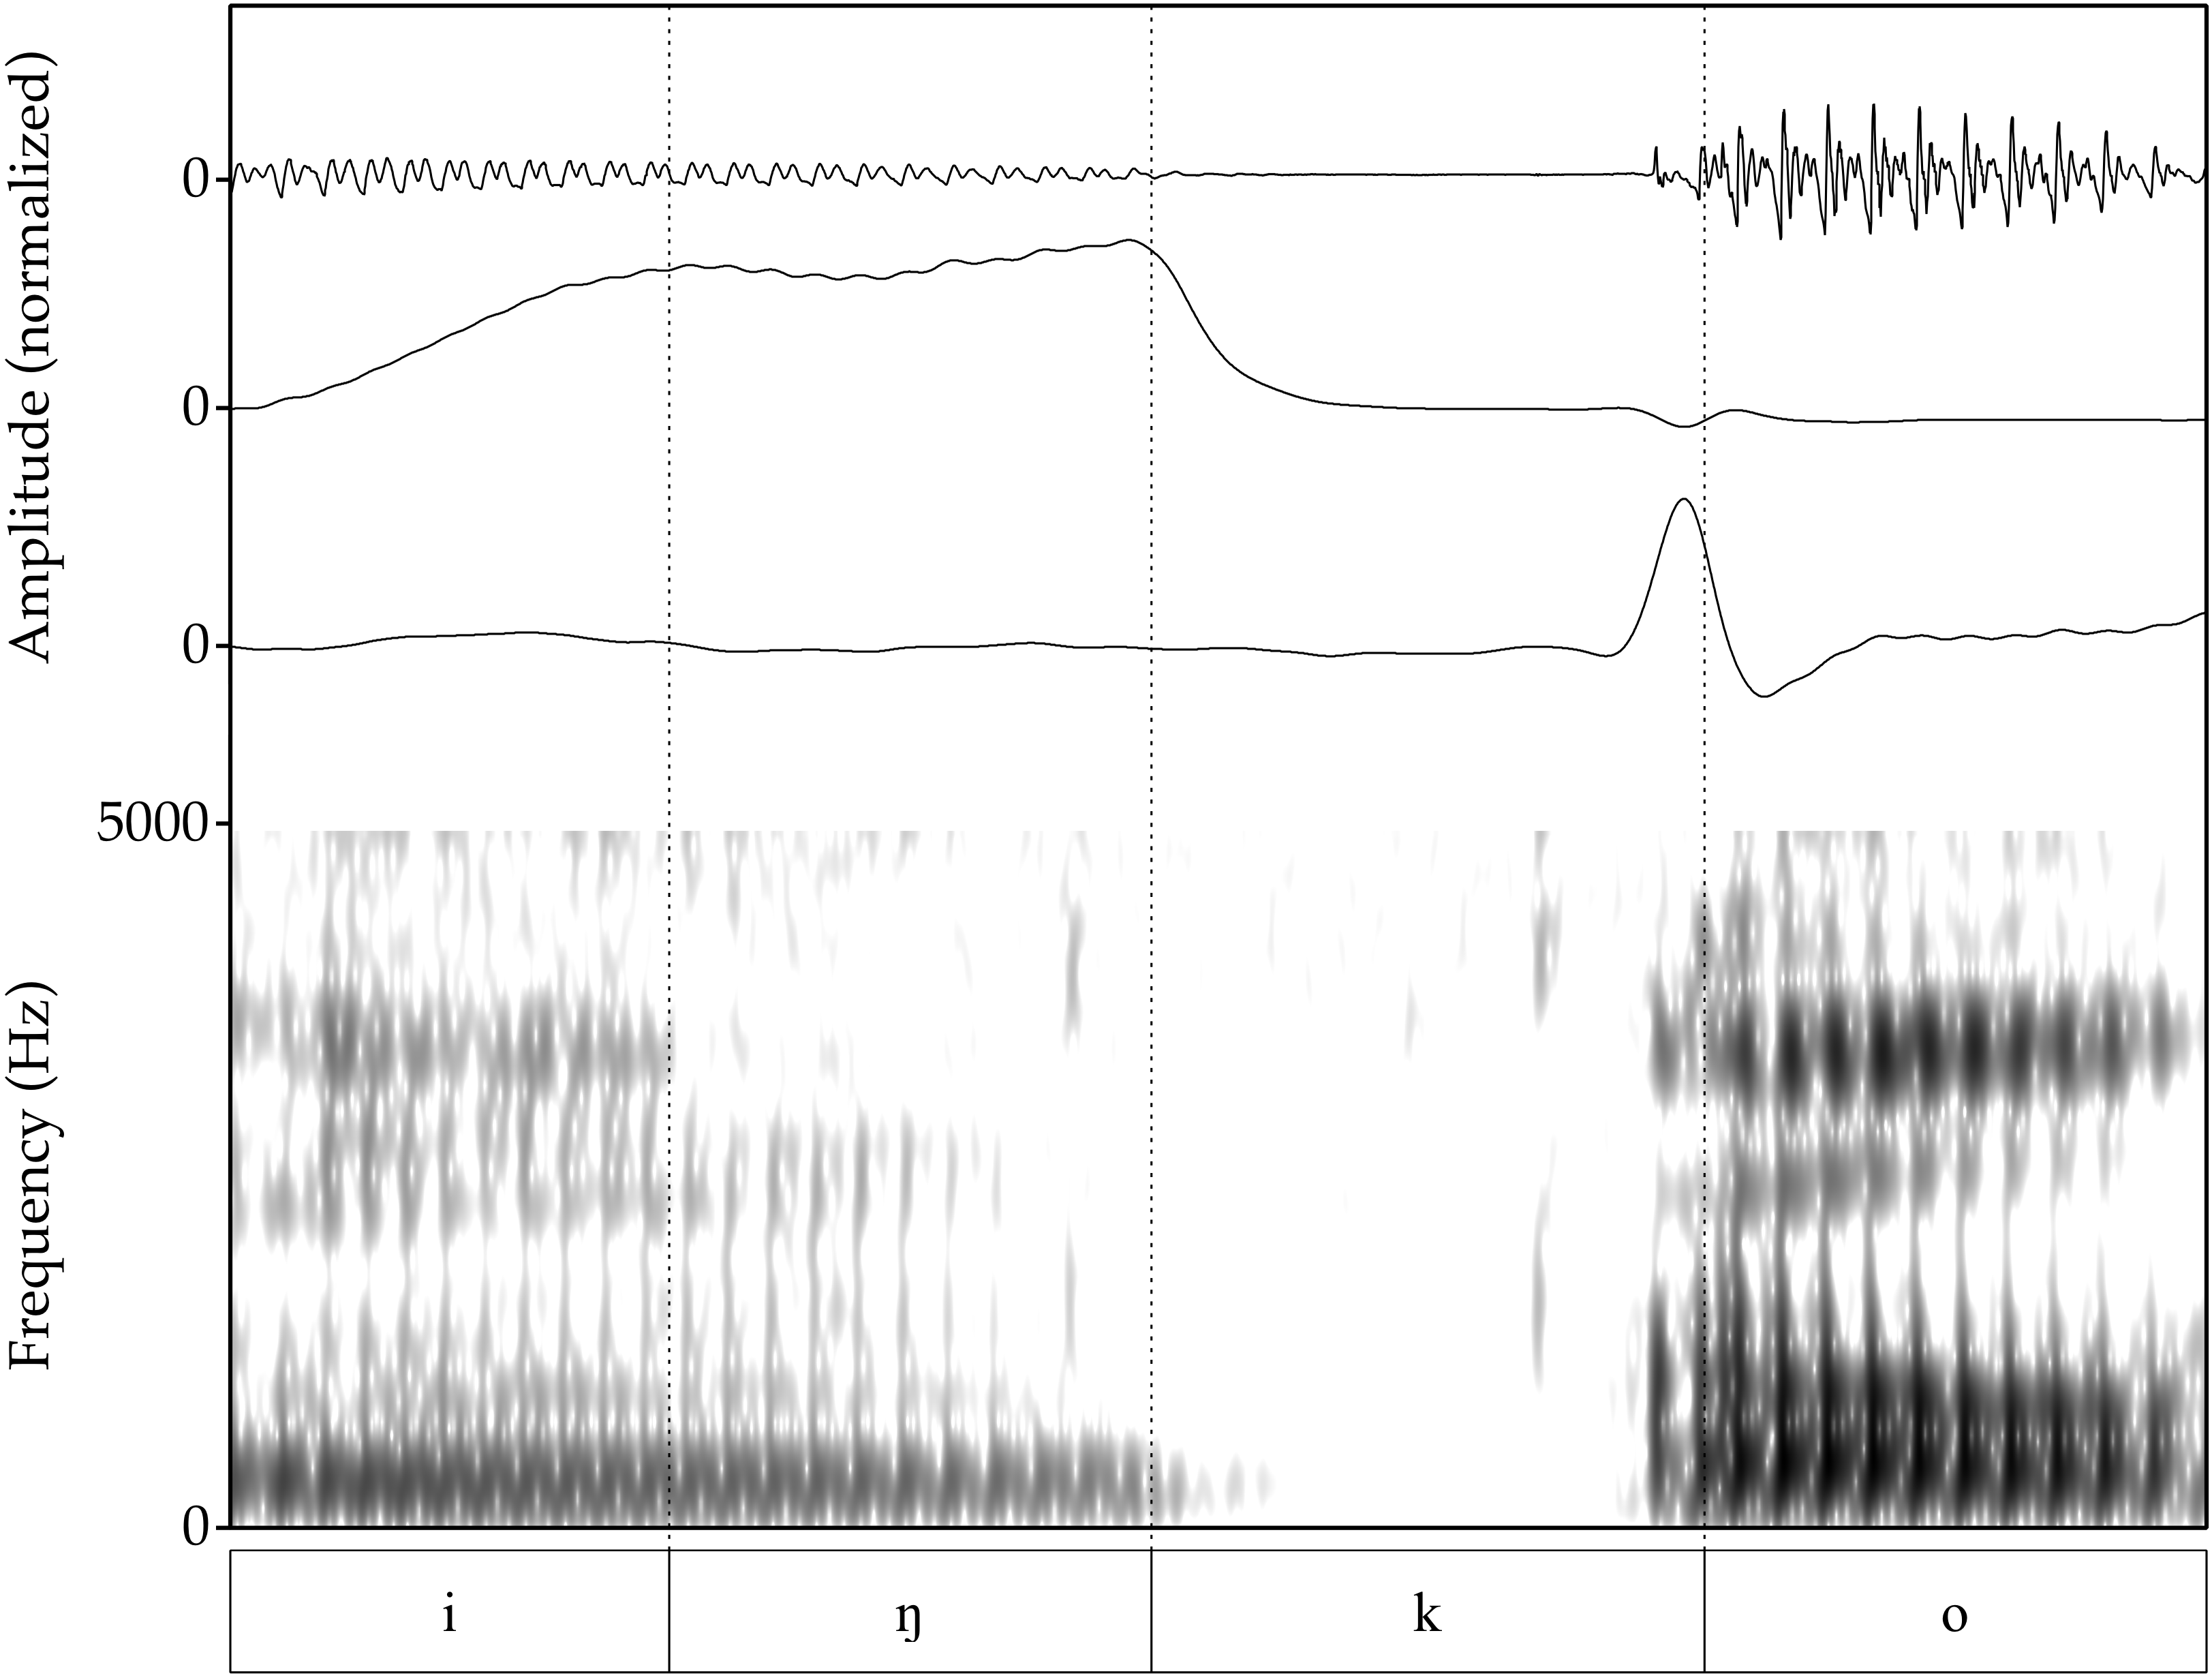
\includegraphics[scale=.8]{figures/inko2.png}
 \caption{Waveform, nasal airflow, oral airflow, and spectrogram (from top to bottom) from the production of the word /ŋo/ [\~iŋko] `water'. Waveform and airflow measures are all normalized from 1 to -1.}
  \label{inko2}
\end{figure}


Figure \ref{inko2} below presents the waveform, nasal airflow, oral airflow, and spectrogram for the production of the word /{\NG}o/ [\~i{\NG}ko]\footnote{The word-initial [\~i] in [\~i{\NG}ko] is an epenthetic vowel that surfaces before root-initial geminates and [NT]s in \ili{Panãra} to satisfy a word-minimality requirement of two syllables. For a full account of this phonological pattern, see \citet{Lapierre2019}.} `water' by a male speaker of \ili{Panãra} (age\,=\,23). As can be observed, vocal fold vibration ceases at the moment that peak nasal airflow is achieved; in other words, vocal fold vibration is suppressed at the moment when the velum is maximally open. As discussed above in \sectref{sec:lapierre:1.2.1}, the natural state of the glottis during an oral stop that occurs after a nasal consonant is for vocal fold vibration to occur; however, it appears that vocal fold vibration is actively suppressed during the oral portion of [NT]s in \ili{Panãra}. From this, I conclude that \ili{Panãra} exhibits a clear and categorical process of synchronic postnasal devoicing.

\section{Evidence of ND $>$ NT in Panãra}\label{sec:lapierre:3}

In this section, I consider two recent proposals for the internal classification of \ili{Jê} and present comparative data from nasal consonants across the family. I argue that the realization of nasal stops between two phonemically oral vowels in \ili{Proto-Jê}, as well as in \ili{Proto-Northern-Jê}, was [mb], with a voiced oral release. Finally, I derive the present-day form of the realization of nasal stops between oral vowels for both family trees. I conclude that a direct sound change from ND $>$ NT must indeed have occurred from \ili{Proto-Northern-Jê} to \ili{Panãra}.

\subsection{The internal classification of Jê languages}

The internal classification of \ili{Jê} languages is a topic of current debate in the \ili{Jê} literature. Two recent proposals for the internal organization of the \ili{Jê} family are presented below in Figures \ref{Lapi} and \ref{Niku}.

\begin{figure}
% %   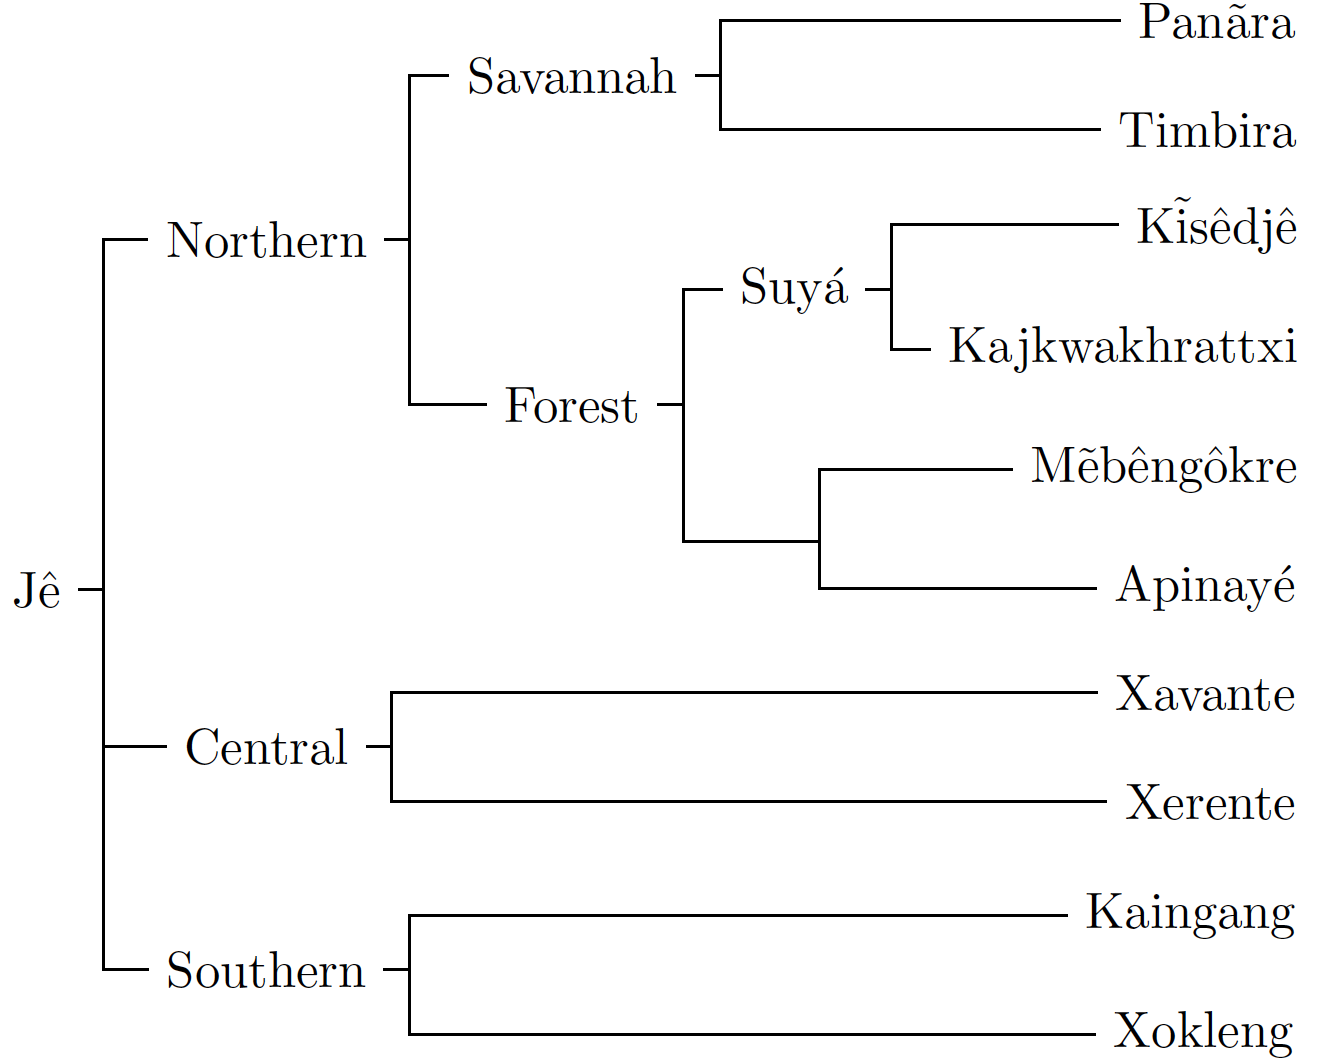
\includegraphics[scale=.33]{figures/TreeLapierreEtAl.png}
    \begin{forest} for tree={grow'=east, forked edges}
     [\ili{Jê}, delay={where content={}{shape=coordinate}{}}
         [Northern\il{Northern-Jê} 
             [Savannah [\ili{Panãra},tier=word] [\ili{Timbira},tier=word]]
             [Forest [\ili{Suyá} [\ili{Kĩsêdjê},tier=word] [\ili{Kajkwakhrattxi},tier=word]]
             [ [\ili{Mẽbêngôkre},tier=word] [\ili{Apinayé},tier=word]]] 
         ]
         [Central\il{Central Jê} [\ili{Xavante}, tier=word] [\ili{Xerente},tier=word]]
         [Southern\il{Southern Jê} [\ili{Kaingang},tier=word] [\ili{Xokleng},tier=word]]
     ]
    \end{forest}
  \caption{First proposal for the subgrouping of Jê \citep{Lapierre2016}}
  \label{Lapi}
\end{figure}
\il{Jê}

\begin{figure}
% %   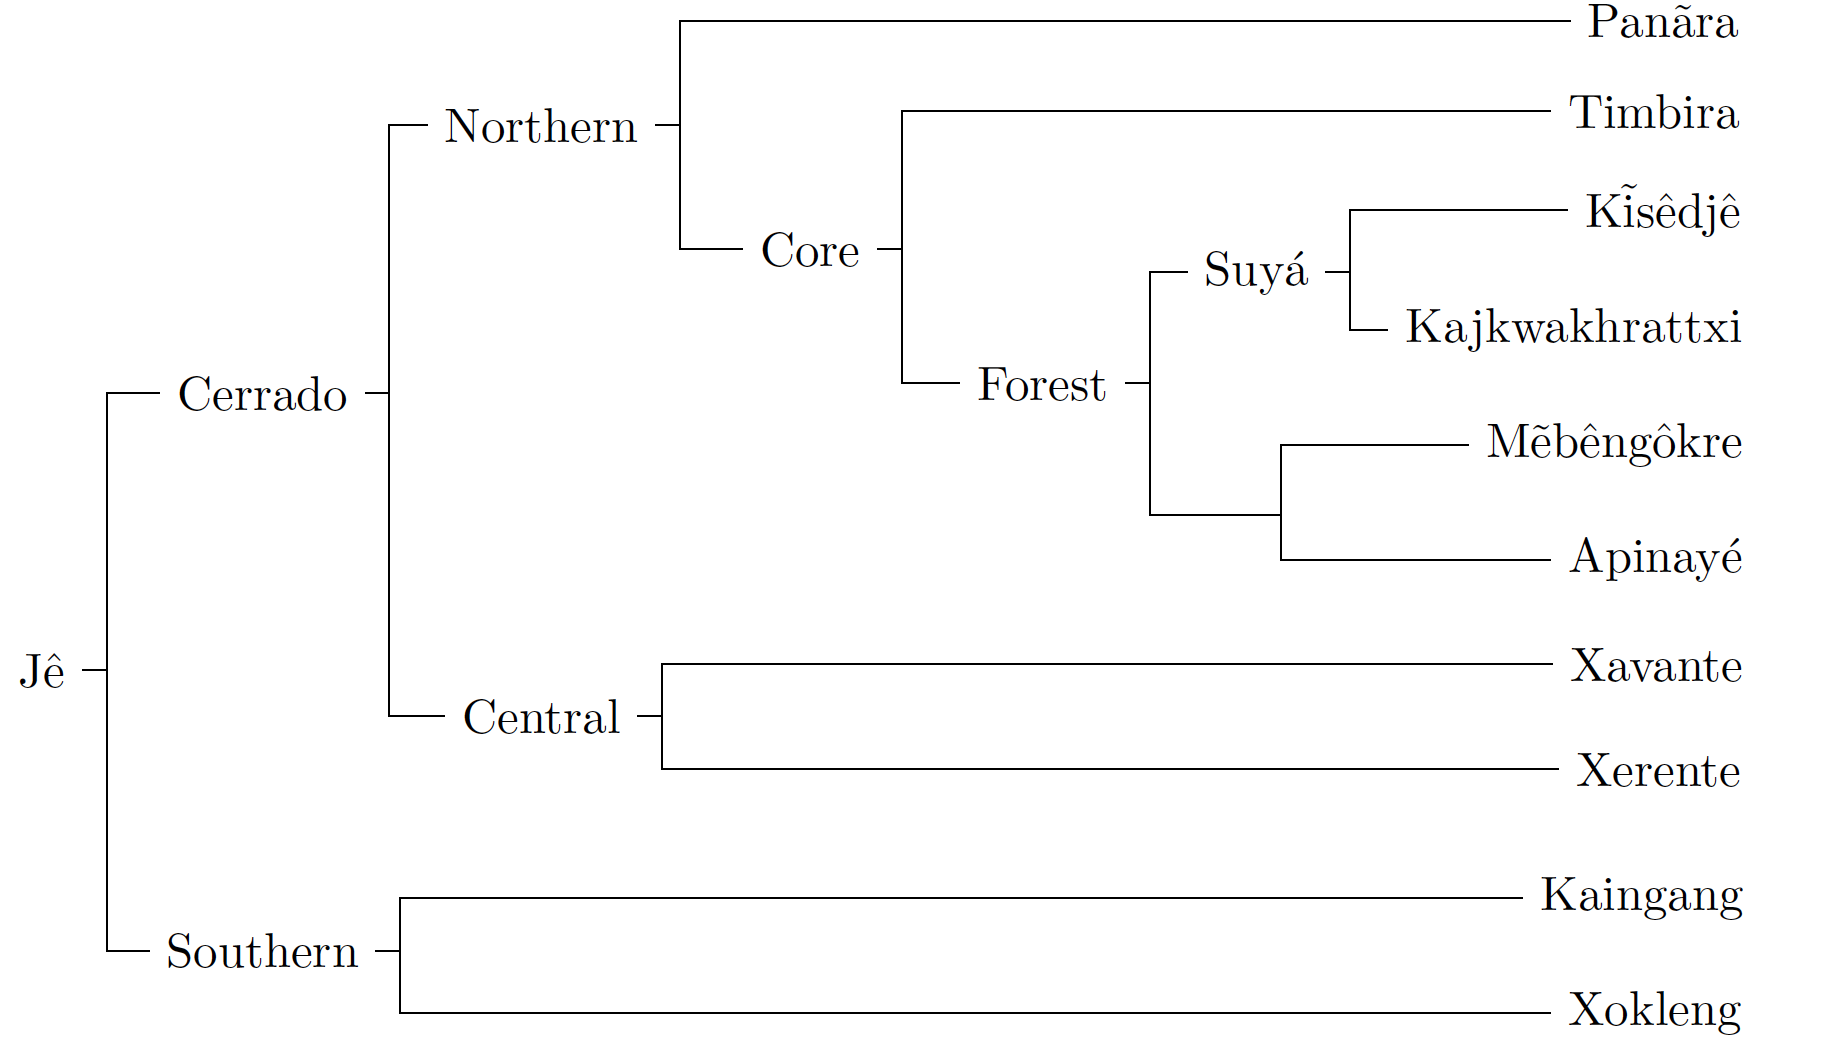
\includegraphics[scale=.34]{figures/TreeNikulin.png}
  \resizebox{\textwidth}{!}{\begin{forest} for tree={grow'=east, forked edges}
     [\ili{Jê}, delay={where content={}{shape=coordinate}{}}
         [\ili{Cerrado} [Northern\il{Northern-Jê} [\ili{Panãra},tier=words]
                     [Core\il{Core Jê} [\ili{Timbira}, tier=words]
                       [Forest [\ili{Suyá} [\ili{Kĩsêdjê},tier=words] [\ili{Kajkwakhrattxi},tier=words]]
                               [ [\ili{Mẽbêngôkre},tier=words] [\ili{Apinayé},tier=words]]
                       ]
                     ]
                   ]
                   [Central\il{Central Jê} [\ili{Xavante}, tier=words] [\ili{Xerente},tier=words]]
         ]
         [Southern\il{Southern Jê} [\ili{Kaingang}, tier=words] [\ili{Xokleng},tier=words]]
     ]     
  \end{forest}}
  \caption{Second proposal for the subgrouping of Jê \citep{Nikulin2016, Nikulin2017}}
  \label{Niku}
\end{figure}


The two proposals crucially differ with respect to the position of \ili{Panãra} and \ili{Timbira} within the \ili{Northern-Jê} subgroup. According to the first proposal (Figure \ref{Lapi}; \citealt{Lapierre2016}), \ili{Panãra} and \ili{Timbira} are sister languages which form a clade separate from the other four \ili{Northern-Jê} languages. According to the second proposal (Figure \ref{Niku}; \citealt{Nikulin2016, Nikulin2017}), \ili{Panãra} was the first language to branch off within \ili{Northern-Jê}, followed by \ili{Timbira}.

Evidence for the classification of \ili{Panãra} and \ili{Timbira} as a clade comes from a number of shared innovations between the two languages that cannot be traced back to \ili{Proto-Northern-Jê}. First, \ili{Panãra} and \ili{Timbira} are the only two \ili{Jê} languages to exhibit a series of contrastive long vowels, as well as a series of contrastive geminate consonants. Both languages underwent a merger, whereby /\~a, \~\textturnv / > /\~\textturnv /, as well as loss of the fully nasalized allophone of the velar nasal. Furthermore, both languages underwent postnasal devoicing, and subsequent denasalization of the resulting [NT] in word-initial position, i.e. ND > NT > T / \# $\underline{\hspace{1em}}$ (see \sectref{sec:lapierre:4.4}. for a discussion of this denasalization process). Finally, they share the change from \ili{Proto-Northern-Jê} /t\textesh / > /s/, followed by /s/ > /h/ in \ili{Timbira} .

Evidence for the classification of \ili{Panãra} as a sister to \ili{Core Jê} comes from Nikulin's claim that the number of innovations in \ili{Panãra} not shared with \ili{Core Jê} is greater than the number of common features between \ili{Panãra} and \ili{Timbira}. He thus proposes that \ili{Panãra} was the first \ili{Northern-Jê} language to split. \ili{Panãra} is the only language where word-final echo vowels became [i], and where word-initial /ka/ simplified to /a/. \ili{Panãra} also underwent changes, whereby {[}{\NG}ɡ\textfishhookr w{]} > {[}{\NG}kw{]}, and /\textfishhookr / > /j/ / $\underline{\hspace{1em}}$ V{[}$+back${]}. Finally, Nikulin proposes that word-initial /ku-/ > /i-/; however, the correct series of sound changes is actually /C$_{1}$C$_{2}$/ > /C$_{2}$ː / > /iC$_{2}$ː /. He further proposes that \ili{Timbira} is the only language where \ili{Proto-Northern-Jê} /t\textesh / > /h/; however, this change almost certainly happened with an intermediate step /t\textesh / > /s/ > /h/, given that /s/ > /h/ is one of the most common sound changes crosslinguistically, and that \ili{Panãra} has /s/ where \ili{Timbira} has /h/. Apinay\'e\il{Apinayé} and \ili{Timbira} underwent metathesis, whereby /\textfishhookr w/ > /w\textfishhookr /, and Apinay\'e\il{Apinayé}, M\~eb\^eng\^okre\il{Mẽbêngôkre} and \ili{Timbira} share the change /tj/ > /t\textesh /.


\subsection{Comparative data from other Jê languages}

In order to determine whether a sound change from ND $>$ NT has occurred in \ili{Jê}, I consider the realization of nasal consonants occurring between two phonemically oral vowels (/N/ $/$ V\longrule V). The relevant synchronic forms are provided in Table \ref{Realization} for all ten \ili{Jê} languages. For the sake of simplicity, the data is presented using the bilabial nasal stop /m/ as a representative example for the full series of nasal consonants, as this general pattern holds for other places of articulation.\footnote{There are some caveats to this generalization. First, \ili{Central Jê} contrasts only two places of articulation for nasal consonants /m, n/, compared to a four-way contrast for the other languages in the family /m, n, \textltailn, {\NG}/. Second, the postoralized allophones of the palatal nasal /\textltailn/ exhibit a lot of variation across the family: \ili{Panãra} [ns]; \ili{Timbira} Ap\~aniekr\'a\il{Apãniekrá} [\textltailn tʃ], K\~is\^edj\^e [\textltailn j, nt], \ili{Kajkwakhrattxi} [nt], M\~eb\^eng\^okre\il{Mẽbêngôkre} [\textltailn], Apinay\'e\il{Apinayé} [\textltailn d\textyogh], \ili{Kaingang} [\textbardotlessj\textltailn\textbardotlessj], and \ili{Xokleng} [nd\textyogh].}


\begin{table}
\caption{Realization of /m/ between two oral vowels in Jê languages}~
\label{Realization}
\begin{tabular}{cccccccccc}
\lsptoprule
{Pan.} & {Tim.} & {Meb.} & {Api.} & {K\~is.} & {Kaj.} & {Xav.} & {Xer.} & {Kai.} & {Xok.} \\
\midrule
{[}mp{]}      & {[}mp{]}      & {[}m{]}       & {[}mb{]}      & {[}mb{]}      & {[}\~wʷ{]}  & {[}b{]}       & {[}b{]}       & {[}bmb{]}     & {[}mb{]}      \\
\lspbottomrule
\end{tabular}
\end{table}
\il{Jê}

The most frequent form observed in the data from Table 2 is [mb], which occurs in 4/10 of the \ili{Jê} languages. [mb] is in fact observed in 5/10 of the languages when one considers the \ili{Kaingang} data in more detail. The data in (\ref{kaingang}) presents the synchronic distribution of nasal stops in \ili{Kaingang} \citep{Wiesemann1972}.

\begin{multicols}{2}
\ea\label{kaingang} a. /m/ $\rightarrow$ [m] $/$ \{\~V, \#\} $\underline{\hspace{1em}}$ \{\~V, \#\} \\
		b. /m/ $\rightarrow$ [mb] $/$ \{\~V, \#\} $\underline{\hspace{1em}}$ V\\
		c. /m/ $\rightarrow$ [bm] $/$ V $\underline{\hspace{1em}}$ \{\~V, \#\}\\
		d. /m/ $\rightarrow$ [bmb] $/$ V $\underline{\hspace{1em}}$ V
		\z
\end{multicols}

\ili{Kaingang} exhibits both a process of postoralization of nasal stops before oral vowels (\ref{kaingang}b), as well as a process of preoralization of nasal stops after oral vowels (\ref{kaingang}c). When a nasal stop occurs between two oral vowels, both postoralization and preoralization take place, resulting in a circum-oralized nasal stop (\ref{kaingang}d). Consequently, \ili{Kaingang} does indeed exhibit an allophone [mb], as is the case for Apinay\'e\il{Apinayé}, K\~is\^edj\^e, \ili{Kajkwakhrattxi}, and \ili{Xokleng}. This pattern is consistent with the implicational hierarchy proposed by \citet{stanton2017}, whereby if a language exhibits circum-oralized nasal stops, it also exhibits postoralized nasal stops (\ref{implication}).

\ea\label{implication} [mb] $>>$ [bmb]
\z

\ili{Kajkwakhrattxi} exhibits an interesting case of shielding, as the postoralized segment is an approximant [\~wʷ], rather than a stop [mb]. This pattern arises because \ili{Kajkwakhrattxi} contrasts oral and nasal bilabial approximants /w, \~w/ \citep{Beauchamp2019} as a result of a historical lenition process that affected all bilabial stops, namely [m, mb, p] > [\~w, \~wʷ, hw]. As observed during my own fieldwork on \ili{Kajkwakhrattxi}, the postoralization of the nasal bilabial approximant is quite perceptually salient. Note that the pattern observed at other places of articulation is different: Nasal velars before oral vowels are always realized as [nɡ], and nasal alveolars before oral vowels exhibit variation between [nd $\sim$ n].

The M\~eb\^eng\^okre\il{Mẽbêngôkre} pattern is the most divergent from the other \ili{Jê} languages, as nasal consonants are realized as fully nasal [m] before oral vowels. Crucially, M\~eb\^eng\^okre\il{Mẽbêngôkre} is the only language that does not exhibit some form of shielding.\footnote{Some authors \citep{StoutThomson1974, SalanovaReisSilva2011} report preoralization of nasal consonants after oral vowels in coda position, such that /m/ $\rightarrow$ [bm] /  V $\underline{\hspace{1em}}$. However, in my own fieldwork with speakers of the Xikr\'in\il{Xikrín} dialect of M\~eb\^eng\^okre\il{Mẽbêngôkre}, I did not observe this process. I also conducted elicitation with speakers of the Kayap\'o\il{Kayapó} dialect of M\~eb\^eng\^okre\il{Mẽbêngôkre}, and I did not observe this process in their speech either.}

Two allophones of /m/ occurring before oral vowels remain to be explained, namely the fully oralized [b] of \ili{Xavante} and \ili{Xerente}, and the postoralized and devoiced [mp] of \ili{Panãra} and \ili{Timbira}. Both of these allophones can be rather straightforwardly accounted for as variants of the shielding process. Specifically, the case of \ili{Xavante} and \ili{Xerente}\footnote{As a very thoughtful reviewer notes, \ili{Proto-Jê} *p and *m underwent a series of sound changes in \ili{Central Jê}, obscuring the correspondences between [p, m] in Central\il{Central Jê} vs. Northern\il{Northern-Jê} and \ili{Southern Jê}. Crucially, *p underwent nasalization before nasal vowels, and *mb underwent complete oralization before oral vowels, and in some cases, devoicing \citep{Davis1966}. As such, \ili{Central Jê} [m] corresponds to both [p, m] in Northern\il{Northern-Jê} and \ili{Southern Jê}, and \ili{Central Jê} [p] corresponds to both [p, m] in Northern\il{Northern-Jê} and \ili{Southern Jê}. These sound changes are summarized in (\ref{aaa}).


\begin{multicols}{2}
\ea\label{aaa} a. *m >  m $/$ $\underline{\hspace{1em}}$ \~V \\
		b. *mb >  b, p $/$ $\underline{\hspace{1em}}$ V \\
		c. *p >  m $/$ $\underline{\hspace{1em}}$ \{]$\sigma$, \~V\} \\
		d. *p >  p $/$ $\underline{\hspace{1em}}$ V
		\z
\end{multicols}


Despite these sound changes, the data that I consider here, namely the realization of /m/ between two oral vowels, only corresponds to \ili{Proto-Jê} *mb. Crucially, the words resulting from (\ref{aaa}a, \ref{aaa}c) are excluded, since the relevant stops occur before nasal vowels. The words resulting from (\ref{aaa}d) are also excluded because they do not correspond to an underlying nasal stop in modern \ili{Central Jê}. Finally, the change in (\ref{aaa}b) resulted in *mb being realized as [b] in some words and as [p] in others. As such, the changes in (\ref{aaa}) do not invalidate the data considered here. While it is true that there are certain cases of \ili{Proto-Jê} *mb that are being excluded from the present analysis (namely those realized as [p] in modern \ili{Central Jê}), the cases that are being considered, namely the [b] reflex of \ili{Proto-Jê} *mb, are the only cases of /m/ occurring between two phonemically oral vowels in modern \ili{Central Jê}.

At this time, I am unable to provide an explanation of the conditioning environment of the two reflexes of *mb in \ili{Central Jê}, [b, p]. \citet{Nikulin2017} proposes that \ili{Xavante} [b] results from a process of stop voicing before high vowels; however, I have not been able to find any evidence of a difference in the realization of voiceless stops before high and non-high vowels in \ili{Central Jê}. In Nikulin's own data, there are a number of cases of \ili{Proto-Jê} *p and *t that are not realized with voicing before high vowels, as well as instances of [b, d] occurring before non-high vowels (p. 160). In \citet{Quintino2000} and \citet{Pickering2010}, there are abundant examples of voiced stops before non-high vowels, as well as of voiceless stops before high vowels.} is one of complete, rather than partial, oralization of nasal consonants (\ref{b}); and the case of \ili{Panãra} and \ili{Timbira}\footnote{There are a number of cases where \ili{Proto-Jê} *mb corresponds to [p] in \ili{Timbira}. This suggests that \ili{Timbira} has undergone a diachronic process of denasalization (*mb > mp > p) affecting most instances of [mp], except those in stem-initial position when preceded by a vowel-final morpheme. The items in which \ili{Proto-Jê} *mb corresponds to \ili{Timbira} [p] are excluded from this analysis, as they cannot synchronically be analyzed as underlying nasals /m/ in the grammar of \ili{Timbira}. Rather, these are now underlying voiceless stops /p/. Furthermore, there are some rare cases where /m/ is realized without postoralization in \ili{Timbira} (e.g. [jama] `chin'), suggesting that postoralization of the type in (\ref{mp}) is no longer productive in \ili{Timbira} grammar.
}
 is one of devoicing of the oral release of the nasal stop (\ref{mp}). 

\begin{multicols}{2}
\ea\label{b} /m/ $\rightarrow$ [b] $/$ $\underline{\hspace{1em}}$ V \z
\ea\label{mp} /m/ $\rightarrow$ [mp] $/$ $\underline{\hspace{1em}}$ V \z
\end{multicols}



Returning now to the question of the most common phonetic realization of nasal consonants before oral vowels in \ili{Jê} languages, I propose that this form is [mb], with postoralization and a voiced oral release. Crucially, postoralization of nasal consonants before oral vowels is observed in 7/10 of the \ili{Jê} languages, and some form of oralization of nasal consonants before oral vowels is observed in 9/10 of the \ili{Jê} languages. For this reason, I reconstruct *mb as the \ili{Proto-Jê} form corresponding to the set of phones in Table \ref{Realization}. All of the other reflexes of *mb, namely [\~wʷ], [bmb], [mp], [b] and [m], can be straightforwardly explained by one of a number of natural sound changes from *mb. These sound changes are presented below in (\ref{change}). \citet{Nikulin2016, Nikulin2017} and \citet{Davis1966} also reconstruct *mb for \ili{Proto-Jê}, indicating some agreement regarding this analysis among \ili{Jê} researchers. In the following subsection, I provide evidence from an earlier variety of \ili{Panãra} supporting a sound change from ND > NT.


\ea\label{change} a. mb $>$ bmb	\hspace{1.01cm}		Preoralization			\hspace{2.7cm}		(\ili{Kaingang})\\
	b. mb $>$ mp	\hspace{1.2cm}		Devoicing of oral release	\hspace{.98cm}	(\ili{Panãra}, \ili{Timbira})\\
	c. mb $>$ b	\hspace{1.51cm}		Complete oralization		\hspace{1.6cm}	(\ili{Xavante}, \ili{Xerente})\\
	d. mb $>$ m	\hspace{1.4cm}		Loss of postoralization	\hspace{1.29cm}		(M\~eb\^eng\^okre\il{Mẽbêngôkre})\\
	e. mb $>$ \~wʷ	\hspace{1.25cm}		Lenition	\hspace{3.53cm}		(\ili{Kajkwakhrattxi})\\
\z

\subsection{Evidence from Southern Cayap\'o}\label{sec:lapierre:3.3}
\begin{sloppypar}
Additional evidence that a sound change from ND > NT occurred in \ili{Panãra} comes from historical documents on Southern Cayap\'o\il{Southern Cayapó}. The Southern Cayap\'o\il{Southern Cayapó} were proposed by \citet{Heelas1979} to be the ancestors of the currently living \ili{Panãra}. This proposal was supported by \citet{Schwartzman1988, RodriguesDourado1993, Giraldin1997, Giraldin2000}, and \citet{Dourado2004}. \citet{Vasconcelos2013} provides a detailed comparison of Southern Cayap\'o\il{Southern Cayapó} data to Apinay\'e\il{Apinayé}, Ap\~aniekr\'a\il{Apãniekrá}, \ili{Kajkwakhrattxi}, and \ili{Panãra} data, and concludes that the language spoken today by the \ili{Panãra} is indeed the same language that was spoken by the Southern Cayap\'o\il{Southern Cayapó}.
\end{sloppypar}

\begin{sloppypar}
Vasconcelos reviews all 7 historical documents available for Southern Cayap\'o\il{Southern Cayapó}. As he points out (p. 134), all but one \citep{Ehrenreich1894} of the documents present evidence of voiced stops in onset of unstressed syllables. This suggests that Southern Cayap\'o\il{Southern Cayapó} likely exhibited variable stop voicing in this phonological environment,
%\footnote{This is consistent with the proposed analysis of M\~eb\^eng\^okre\il{Mẽbêngôkre} voiced stops, according to which /b, d, \textdyoghlig, \textscriptg/ phonologized in the onset of unstressed syllables.}
e.g. Southern Cayap\'o\il{Southern Cayapó} <impute $\sim$ impude> [\~im.\textprimstress pu.te $\sim$ \~im.\textprimstress pu.de] and \ili{Panãra} [\~im.\textprimstress puː.ti] `neck'.
%Southern Cayap\'o\il{Southern Cayapó} <rob\'u> [\textprimstress\textfishhookrɔ.bɯ] and \ili{Panãra} [\textprimstress jɔː.pɯ] `dog'
Furthermore, although the vast majority of transcriptions in these documents suggest that the oral release of postoralized nasals was generally voiceless, three documents provide evidence of some instances of [ND]s. Vila Boa's 1782 baptism registry\footnote{This historical data was accessed through \citet{Vasconcelos2013}.} contains a list of proper names that present postoralized nasals, both voiced [mb] ($n=5$\footnote{<Angrayocha, Pembaque, Ungaptuai, Combono, Cambriopixom>}) and voiceless [mp] ($n=18$\footnote{<Queampia, Coimpa, Uncrixiu, Xuanampiae, Carampea (x2), Incapuim, Quipanto, Encon\^a, Tuuntu, Tanquer\'e, Emponi, Xampeu, Canampuaxi, Xampea, Cananquete, Tuinta, Canampui>}), suggesting that these two sounds were likely in variation at the time that the document was written. \citet{LemosdaSilva1882}, accessed through \citet{Vasconcelos2013}, presents one lexical item suggesting the presence of a voiced [mb].\footnote{<copembe> `acabou,' (Vasconcelos' proposed IPA transcription [k\~op\~embe])} \citet{Barbosa1918} presents a number of <mb, nd> transcriptions.\footnote{<ambrend\'a> `dois,' <iund\'e> `atravessar,' <iund\^e> `compadre,' <tapyund\'e> `arrependerse,' <iund\^ek\'ua> `comadre'.} Note that the historical data from Vila Boa, Lemos da Silva, and Barbose was accessed through \citet{Vasconcelos2013}.
\end{sloppypar}

The data from these historical documents thus suggest that Southern Cayap\'o\il{Southern Cayapó} exhibited some variation between voiced and voiceless postoralized nasal stops. Since this variation is no longer observed in \ili{Panãra}, the data presented here support the claim that a sound change from ND > NT did indeed occur in an earlier variety of the language. Furthermore, transcriptions of plain voiced stops D occur more frequently in these historical documents than do transcriptions of ND, suggesting that postnasal devoicing (ND > NT) probably happened before plain stop devoicing (D > T), and that an analysis positing across-the-board devoicing of stops (*D) as a single sound change is likely incorrect (see \sectref{sec:lapierre:4.1}).

\subsection{Evidence from Macro-Jê languages}

Further evidence that a sound change from ND > NT did occur in \ili{Panãra} comes from comparative data from \ili{Macro-Jê} languages. A list of the following 12 \ili{Macro-Jê} languages was compiled by referring to the SAPhon database \citep{saphon}: B\'es\textbari ro\il{Bésɨro}, \ili{Bororo}, Guat\'o\il{Guató}, Djeoromitx\'i\il{Djeoromitxí}, Arikap\'u\il{Arikapú}, Karaj\'a\il{Karajá}, Kren\'ak\il{Krenak}, Ofay\'e\il{Ofayé}, Pur\'i\il{Purí}, Maxakal\'i\il{Maxakalí}, Rikbaktsa, and \ili{Yaathe}. Of this set of languages, five exhibit shielding. Specifically, Arikap\'u\il{Arikapú} \citep{RibeiroVoort2010}, Kren\'ak\il{Krenak} \citep{Pessoa2012}, and Maxakal\'i\il{Maxakalí} \citep{Campos2009} exhibit [mb] before oral vowels and [m] before nasal vowels. Furthermore, Djeoromitx\'i\il{Djeoromitxí} \citep{RibeiroVoort2010} and Karaj\'a\il{Karajá} \citep{Ribeiro2012} exhibit [b] before oral vowels and [m] before nasal vowels. Note that none of the \ili{Macro-Jê} language exhibits shielding of the type observed in \ili{Panãra}, with a voiceless oral portion. There is thus no clear evidence suggesting that *mp should be reconstructed for \ili{Proto-Macro-Jê}, but there is some support for the reconstruction of *mb as the realization of nasal stops occurring before oral vowels in \ili{Proto-Macro-Jê}. Furthermore, if \ili{Proto-Macro-Jê} did have voiceless postoralized nasals, we would perhaps expect to find more languages of the family to retain [NT]. However, this is not the case.

\subsection{Deriving the sound changes}

In this subsection, I derive the synchronic reflexes of \ili{Proto-Jê} *mb for each of the ten extant \ili{Jê} languages according to the two subgrouping proposals in Figures \ref{Lapi} and \ref{Niku}. I begin this discussion by mapping out the possible sound changes that can occur between the synchronic reflexes of *mb in each one of the ten \ili{Jê} languages, namely [mb, m, \~wʷ, bmb, b, mp, p] (Figure \ref{statemap}).

\begin{figure}
% %   
\includegraphics[scale=.35]{figures/ChangeOfState7.png}
  \begin{tikzpicture}[>=Triangle]
  \matrix [matrix of nodes, row sep=.75cm, column sep=1cm, nodes={font={\strut}}] 
  (matrix) {     & b  & p\\
             bmb & mb & mp\\
             \~{w}\textsuperscript{w} & & m\\};
  \draw[->] (matrix-2-1) -- (matrix-1-2);
  \draw[<->] (matrix-1-2) -- (matrix-1-3);
  \draw[<->] (matrix-1-2) -- (matrix-2-2);
  \draw[<->] (matrix-1-3) -- (matrix-2-3);
  \draw[<->] (matrix-2-2) -- (matrix-2-3);
  \draw[<->] (matrix-2-1) -- (matrix-2-2);
  \draw[<->] (matrix-3-1) -- (matrix-2-2);
  \draw[<->] (matrix-3-3) -- (matrix-2-2);
  \end{tikzpicture}
  \caption{Possible sound changes between [mb, m, \~wʷ, bmb, b, mp, p]\label{statemap}}
\end{figure}

The arrows in Figure \ref{statemap} present what I consider to be possible sound changes between the seven sounds. Specifically, a sound change is considered possible if (1) it is attested, and/or (2) it involves a change in a single phonetic feature. If a sound change is unattested, or if it involves a change in more than one feature at a time (i.e., if it is saltatory, \citealt{HayesWhite2015}), then I consider that sound change impossible. The changes presented in (\ref{14}--\ref{15}) involve changes in two phonetic features at once, and are thus considered impossible as a single sound change. While some of the changes in (\ref{14}--\ref{17}) may have occurred, these are assumed to have been telescoped through a sequence of two (or more) changes. (\ref{18}) is unattested.

\ea\label{14} a. m $>$ mp\footnote{Apart from \ili{Panãra} and \ili{Timbira}, all other attested cases of postoralization of a nasal consonant involve a voiced oral release, e.g., [mb].} 	\hspace{.8cm} 			Postoralization and devoicing of oral release \\
b. mp $>$ m	\hspace{1.06cm}			Voicing of oral release and postnasalization
\ex\label{15} a. m $>$ bmb	\hspace{.88cm}			Preoralization and postoralization	\\
b. bmb $>$ m\footnote{This change is unattested. All languages that exhibit circum-oralized [bmb] also exhibit [mb] (\ref{implication}). It is thus assumed that the presence of [bmb] must be preceded by [mb], i.e. mb $>$ bmb.} 	\hspace{.60cm}			Prenasalization and postoralization	
\ex\label{16} a. b $>$ mp	\hspace{1.17cm}			Prenasalization and devoicing	\\
	b. mp $>$ b\footnote{While there are many attested cases of changes from mp $>$ b, I assume that this happens through telescoping of an intermediate stage, i.e., mp $>$ mb $>$ b.} 	\hspace{.89cm}			Oralization and voicing
\ex\label{17} a. m $>$ \~wʷ	\hspace{1.06cm}			Postoralization and lenition	\\
	b. \~wʷ $>$ m\footnote{I assume here that any change between [m] and [\~wʷ] must be telescoped through [\~w]. Note that a change from m > \~w is in fact attested in \ili{Kajkwakhrattxi}.} 	\hspace{.75cm}			Postnasalization and fortition
\ex\label{18} b $>$ bmb\footnote{Cases of prenasalization (b $>$ mb) and postnasalization (b $>$ bm) are common in the literature \citep{WetzelsNevins2018}; however, cases of medio-nasalization (b $>$ bmb) are unattested.} 	\hspace{1.05cm}			Medio-nasalization
\z


Assuming the internal classification proposed by \citet{Lapierre2016}, it is necessary to posit five independent sound changes in order to derive the present day realization of /m/ between two oral vowels in the ten extant \ili{Jê} languages. Specifically, the following sound changes must have occurred: (1) mb $>$ bmb in \ili{Kaingang}; (2) mb $>$ b in \ili{Central Jê}; (3) mb $>$ mp in Savannah \ili{Jê}; (4) mb > \~wʷ in \ili{Kajkwakhrattxi}; and (5) mb $>$ m in M\~eb\^eng\^okre\il{Mẽbêngôkre}. Other potential pathways are possible to arrive from *mb to the present-day forms in the ten \ili{Jê} languages, but these would require a greater number of posited sound changes. Because all of these other conceivable sequences of events are less parsimonious than the one presented here, I do not discuss them.

\begin{sloppypar}
I now consider two possible ways in which it is possible to derive the present day realization of /m/ between two oral vowels in the ten modern \ili{Jê} languages, assuming the subgrouping proposed by \citet{Nikulin2016, Nikulin2017}. The first set of changes involves six independent sound changes, including two instances of mb $>$ mp, and the second set of sound changes involves seven independent innovations, including two cases of mb $>$ mp $>$ mb back-mutation. The first set of possible sound changes that can derive the present day forms of \ili{Proto-Jê} *mb includes: (1) mb $>$ bmb in \ili{Kaingang}; (2) mb $>$ b in \ili{Central Jê}; (3) mb $>$ mp in \ili{Panãra}; (4) an additional independent change from mb $>$ mp in \ili{Timbira}; (5) mb > \~wʷ in \ili{Kajkwakhrattxi}; and (6) mb $>$ m in M\~eb\^eng\^okre\il{Mẽbêngôkre}. Given that homoplasy is known to occur \citep{Chang2015}, having to posit two independent instances of postnasal devoicing within \ili{Northern-Jê} may not be so controversial. However, the change from mb $>$ mp is, at best, typologically rare (see \sectref{sec:lapierre:1}), and it seems suboptimal to have to posit two independent changes from mb $>$ mp. 
\end{sloppypar}

The second set of possible sound changes that can derive the present day forms of \ili{Proto-Jê} *mb includes: (1) mb $>$ bmb in \ili{Kaingang}; (2) mb $>$ b in \ili{Central Jê}; (3) mb $>$ mp in \ili{North-Western Jê}; (4) two cases of back-mutation from mp~$>$~mb in \ili{Core Jê}; (5) mb > \~wʷ in \ili{Kajkwakhrattxi}; and (6) mb $>$ m in M\~eb\^eng\^okre\il{Mẽbêngôkre}. While this set of sound changes has the advantage of positing a single instance of mb~$>$~mp, it is less parsimonious than the other set of changes presented above, as it includes an additional sound change, and it further includes two cases of back-mutation from mb $>$ mp $>$ mb. 

It is unclear which of the two sets of sound changes proposed for Nikulin's subgrouping would be more likely to have occurred. Nevertheless, both of the proposed pathways for Nikulin's subgrouping of \ili{Jê} are suboptimal compared to the sequence of events that must be posited when assuming Lapierre et al.'s subgrouping, as the series of four sound changes proposed for Lapierre et al.'s subgrouping is the most parsimonious way to derive the present-day realization of /m/ in the ten modern \ili{Jê} languages. Of course, in order to determine which of the two \ili{Jê} subgroupings is most likely, we must consider a much larger set of evidence than simply the changes of state of \ili{Proto-Jê} *mb, but the evidence presented here does support Lapierre et al.'s subgrouping. Regardless of which phylogenetic proposal is correct, the crucial point here is simply that a sound change from ND $>$ NT must have occurred \textit{at least once} in the history of the \ili{Jê} languages, and that this must have occurred as a single sound change.

\section{Discussion}
\subsection{One or more sound changes?}\label{sec:lapierre:4.1}

In \sectref{sec:lapierre:3}, I argued that a change from ND $>$ NT must have occurred in \ili{Panãra} and \ili{Timbira}. The proposal that this occurred as a single sound change, rather than as a series of telescoped sound changes, appears, at first glance, to challenge \citegen{Begus2019} proposal for the Blurring Process (\ref{blurring}); however, I show here that this is not in fact the case.

Additional evidence that ND $>$ NT in \ili{Panãra} and \ili{Timbira} occurred as a single sound change comes from the absence of a series of voiced stops in \ili{Proto-Jê} \citep{Davis1966}.\footnote{\citet{Nikulin2016, Nikulin2017} posits a series of voiced stops (*b, *\textbardotlessj, *\textscriptg) for \ili{Proto-Northern-Jê}. The author claims that voiced stops underwent devoicing in all of the \ili{Northern-Jê} languages except M\~eb\^eng\^okre\il{Mẽbêngôkre}, the only \ili{Northern-Jê} language to exhibit voiced stops. This proposal, however, is implausible. As \citet{WetzelsNevins2018} clearly note, languages with a three-way stop contrast /m, b, p/ do not exhibit shielding. If a language had a three-way stop contrast, shielding would not result in contrast \textit{enhancement}, but rather in reduction of the /m, b/ contrast. Since, to the best of my knowledge, no such language is attested, the proposal that \ili{Proto-Northern-Jê} exhibited a series of voiced stops as well as shielding is improbable. I follow \citet{Davis1966} in assuming that the voiced stops in M\~eb\^eng\^okre\il{Mẽbêngôkre} are an innovation. While the details of the motivation for this innovation are not clear, all voiced stops in the language seem to be predictable. First, /\textdyoghlig / is the reflex of \ili{Proto-Northern-Jê} *t\textesh\space ([s] in \ili{Panãra} and K\~is\^edj\^e\il{Kĩsêdjê}, [t] in \ili{Kajkwakhrattxi}, [t\textesh] in Apinay\'e\il{Apinayé}, and [h] in \ili{Timbira}), since /\textdyoghlig / is the most common of the voiced stops in M\~eb\^eng\^okre\il{Mẽbêngôkre} and /t\textesh/ is very marginal (p.c. Salanova 2016). Furthermore, /d, \textscriptg / are very marginal and seem to only occur in function words. /b/ is more common than /d, \textscriptg / but also seems to occur more frequently in function words and in the onset of unstressed syllables. As such, I propose that /b, d, \textscriptg / arose as the result of stop voicing in the onset of unstressed syllables, but more methodical comparisons are in order to support this hypothesis. Furthermore, note that M\~eb\^eng\^okre\il{Mẽbêngôkre} is the only \ili{Jê} language to exhibit a series of voiced stops, and also the only \ili{Jê} language that does not exhibit shielding. These two facts seem crucially related (as noted by Wetzels \& Nevins), such that the innovation of the voiced stops likely resulted in the loss of shielding.} According to the Blurring Process, a series of voiced stops first had to undergo spirantization for postnasal devoicing to occur. However, none of the \ili{Jê} languages exhibits a full series of fricatives, and voiced fricatives are absent altogether.\footnote{With the exception of /ð/ in \ili{Xokleng}, and /z/ in \ili{Central Jê}, sometimes realized as [dz] by older \ili{Xavante} speakers} If the change from ND $>$ NT had been telescoped through the sound changes D $>$ Z $>$ D, we would expect to find in those languages that exhibit postnasal devoicing either a series of voiced fricatives, or a series of voiced stops. However, with the exception of voiced stops in M\~eb\^eng\^okre\il{Mẽbêngôkre}, neither a series of voiced stops nor fricatives is observed in any \ili{Jê} language. Thus, neither the diachronic nor the synchronic data from \ili{Jê} presents any evidence of a change from D $>$ Z, or from Z $>$ D, and I conclude that the change from ND $>$ NT did indeed occur as a single sound change.

That said, the data from \ili{Jê} do not present a clear counterexample to the Blurring Process. Begu\v{s} defines postnasal devoicing as a process that applies to voiced stops only after nasals (i.e., D $\rightarrow$ T / N $\underline{\hspace{1em}}$). Crucially, because voiced stops do not occur elsewhere in the grammar of \ili{Panãra} or \ili{Timbira}, the sound change from ND $>$ NT could perhaps be analyzed as a case of unconditioned devoicing (i.e., D $>$ T) banning all voiced stops. This across-the-board ban on voiced stops can be formalized in Optimality Theory as an undominated *D constraint, and would thus not be expected to arise from a series of changes. That said, the historical documents from Southern Cayap\'o\il{Southern Cayapó} suggest that postnasal devoicing may have occurred before the devoicing process for plain stops, as noted in \sectref{sec:lapierre:3.3}. Further investigation is needed to determine whether stop devoicing occurred as a single sound change (D > T) or as two independent changes (ND > NT followed by D > T). Regardless of the correct occurrence of events, this case of postnasal devoicing is especially noteworthy for a number of reasons.

First, this sound change is an instance of a direct change from ND $>$ NT and thus contributes to the body of literature on postnasal devoicing, a change characterized as unnatural by many authors. Second, previously described cases of postnasal devoicing involve a sequence of two phonemes /ND/, where /D/ is realized as [T]. The case described here differs in a crucial way: In \ili{Panãra} and \ili{Timbira}, [NT]s are monosegmental, as they are allophones of the phoneme /N/. Finally, to the best of my knowledge, the synchronic pattern whereby nasal consonants are simultaneously postoralized \textit{and} devoiced (/N/ $\rightarrow$ [NT] / $\underline{\hspace{1em}}$ V) has not yet been discussed. If not unattested, these cases are, at best, very rare.


\subsection{Is ND $>$ NT a phonetically-grounded sound change?}\label{sec:lapierre:4.2}

A sound change may be phonetically-grounded according to either articulatory or perceptual principles. I begin this discussion by considering the articulatory motivation for a change from ND $>$ NT. As discussed in \sectref{sec:lapierre:1.2.1}, aerodynamic principles cause oral stops occurring after nasal consonants to be realized with vocal fold vibration, unless special articulatory effort is made to prevent voicing. However, \citet[104]{Begus2019} notes that ``[d]espite nasal leakage and volume expansion, [...] speakers still need to accommodate for voicing [...] in order to counter the anti-voicing effect of closure---even in postnasal position.'' Devoicing of an oral stop thus has an articulatory motivation, even after nasals. 

The data from \ili{Panãra}, however, does not support an articulatory motivation for the change from ND $>$ NT. Crucially, the nasal airflow measurements presented in Figure \ref{inko2} show that vocal fold vibration ceases at the precise moment when peak nasal airflow is achieved during the production of [NT]. This means that voicelessness of the oral portion of [NT] is not achieved by simply lengthening the oral closure; otherwise, we would expect voicing to persist into the closure of the oral stop and cease at the moment when the air pressure in the oral cavity equalizes with the subglottal cavity. Instead, the airflow data suggests that vocal fold vibration is actively suppressed at the moment when the velum is maximally open, supporting a non-articulatory motivation for the sound change.

An alternative explanation of this sound change is grounded in perceptual principles. Whether a change from ND $>$ NT can be explained by perceptual salience is somewhat controversial, as no experimental evidence has addressed this question directly. Some authors, such as \citet{Hyman2001}; and \citet{Begus2019} argue against a perceptual motivation for postnasal devoicing, but others, such as \citet{Kirchner2000} and \citet{stanton2017} argue in favour of such an explanation. In her typological review of NC segments, Stanton discusses the perceptual cues to the /N, ND/ contrast, namely intrinsic cues (i.e., cues found during the production of the consonant itself), and extrinsic cues (i.e., coarticulatory cues found on neighboring segments). Intrinsic cues to the /N, ND/ contrast are the presence of an oral closure and release during the production of ND, and its absence during the production of N. Extrinsic cues to this contrast are the presence of an oral vowel following ND, and the presence of a nasal vowel following N. Stanton further argues that NT has a more perceptually salient release burst than ND, and that ND has a more perceptually salient release burst than N, as in (\ref{burst}). This proposal is supported by data from a perception experiment on [NT] segments in \ili{Panãra}, which suggests that the voiceless oral release is indeed very perceptually salient to native speakers of the language \citep[]{LapierreLin2019}.

\ea\label{burst} NT $>>$ ND $>>$ N \z

There are two possible ways to increase the perceptual distance between N and ND: Increasing the duration of the oral closure, or devoicing the release burst. These two strategies, however, are not independent (see \sectref{sec:lapierre:1.2.1}). Specifically, the longer the closure of the oral portion, the more likely the burst will be voiceless; conversely, producing a voiceless oral release is likely to result in lengthening of the oral closure, as predicted by the aerodynamic voicing constraint \citep{Ohala1983, Ohala2011}. If these assumptions are true, the two possible pathways for a sound change from ND $>$ NT, as motivated by a need to increase the perceptual distance between N and ND, are (1) lengthening the oral closure of the stop, subsequently leading to a devoicing of the oral release, or (2) devoicing of the oral release, subsequently leading to a lengthening of the oral closure.

The airflow data in Figure \ref{inko2} supports the perceptual account of the ND $>$ NT sound change in \ili{Panãra}. Specifically, vocal fold vibration is actively suppressed at the moment of maximal velic opening, supporting the idea that vocal fold vibration is inhibited to increase the perceptual salience of the oral burst. In addition, the acoustic duration measurements in Table \ref{resultstable} suggest that the oral closure of \ili{Panãra} [NT]s are indeed very long. However, given that vocal fold vibration is actively suppressed, it does not appear that the lengthening of the oral closure arose as a way of inhibiting voicing. Instead, lengthening of the oral closure may be another form of perceptual enhancement of the oral portion of [NT].

Whether sound changes can be motivated by a need for contrast enhancement is controversial. \citet[205]{blevins2004} argues that pressures for contrast enhancement can trigger hyperarticulation, thus avoiding common instances of phonetic mergers (see also \citealt{Flemming2002, Flemming2008a, Flemming2008b} on the role of contrast in grammar). This claim is well supported by experimental results by \citet{BaeseBerkGoldrick2009}, which showed that words with minimal pair neighbours (e.g., \textit{pox} and \textit{box}) were consistently produced with longer VOTs than words without (e.g., \textit{posh} and *\textit{bosh}). This form of lexically conditioned variation suggests that speakers do indeed enhance the phonetic cues to highlight phonemic contrast when these cues serve to distinguish words in the lexicon. 

The case of ND $>$ NT can be viewed as a case of dissimilatory hyperarticulation, since ND $>$ N (as occurred in M\~eb\^eng\^okre\il{Mẽbêngôkre}) results in a partial merger of the contrast between oral and nasal vowels. In contrast, the change from ND $>$ NT results in enhancement of the contrast between oral and nasal vowels. Blevins claims that sound changes that are motivated by contrast enhancement may only arise when there exists free variation between two existing forms. In the case of ND $>$ NT described here for \ili{Panãra}, we expect free variation between [ND] and [NT] to have occurred at an earlier stage of the language. That such variation existed in Southern Cayap\'o\il{Southern Cayapó} is supported by the historical data presented in \sectref{sec:lapierre:3.3}. As such, the proposal that the change from ND $>$ NT in \ili{Panãra} and \ili{Timbira} was perceptually motivated by a need to enhance the contrast between oral and nasal vowels is supported. 

\subsection{Two necessary preconditions for a change from ND $>$ NT}
\begin{sloppypar}
As discussed in \sectref{sec:lapierre:1.2}, only 1.33\% of the languages in UPSID possess NT segments in their phonological inventory. If a change from ND $>$ NT is phonetically-grounded as argued in \sectref{sec:lapierre:4.2}, then why are instances of this change so typologically rare? The change from ND $>$ NT in \ili{Panãra} and \ili{Timbira} appears to be correlated with two characteristics of the languages' phonological systems: (1) the two-way contrast between /N, T/; and (2) the contrast between oral and nasal vowels /V, \~V/. If these two characteristics of the phonemic inventory of a language are prerequisites to the occurrence of a direct sound change from ND $>$ NT, this could explain why this change, as observed in \ili{Panãra}, occurs so infrequently. Crucially, it has been claimed that shielding may only occur in languages that (1) do not exhibit a three-way contrast in stops /N, D, T/ \citep{WetzelsNevins2018}, and (2) exhibit a contrast in oral and nasal vowels \citep{Hyman1975, herbert1986, stanton2017}. I first consider Wetzels \& Nevins' claim.
\end{sloppypar}

Of the ten \ili{Jê} languages, none exhibits both postoralization ([ND] or [NT]) and phonemic voiced stops (/D/). Within the family, none of the languages that exhibit postoralization ([ND] or [NT]) have voiced stops (/D/) (i.e., \ili{Panãra}, \ili{Timbira}, Apinay\'e\il{Apinayé}, K\~is\^edj\^e, \ili{Kajkwakhrattxi}, \ili{Kaingang}, and \ili{Xokleng}), and M\~eb\^eng\^okre\il{Mẽbêngôkre}, the only language with voiced stops /D/, does exhibit shielding. This is well predicted by Wetzels \& Nevins' analysis of the cross-linguistic distribution of postoralized nasal stops, according to which shielding may only occur in languages that do not exhibit a contrastive series of voiced stops.

These typological observations, however, make no prediction as to whether the postoralized allophones should be realized with a voiced or voiceless oral release (i.e., as [ND] or [NT]). Crucially, within \ili{Jê}, only \ili{Panãra} and \ili{Timbira} exhibit voiceless postoralized nasals [NT], while Apinay\'e\il{Apinayé}, K\~is\^edj\^e, \ili{Kajkwakhrattxi}, \ili{Kaingang}, and \ili{Xokleng} all exhibit voiced postoralized nasals [ND]. There seems to be no correlation between the observation that a language does not exhibit phonemic voiced stops and that it exhibits postoralized and devoiced nasals [NT]. Given these facts, it seems unsatisfactory to justify the diachronic change from ND $>$ NT as an instance of across-the-board stop devoicing (*D), as this analysis does not provide an explanation for why such a change \textit{did} occur.

I now turn to the second claim regarding the presence of postoralized nasal consonants, namely that the synchronic process whereby /N/ $\rightarrow$ [{ND, NT}] / $\underline{\hspace{1em}}$ V may only occur in languages that license a contrast between oral and nasal vowels \citep{Hyman1975, herbert1986, stanton2017}. In a language that does not exhibit shielding, nasal consonants are realized as fully nasal before phonemically oral vowels, which results in some coarticulatory nasalization of the following vowel (/ma/ $\rightarrow$ [m\textsuperscript{\~a}a]). Given that an intrinsic cue to the contrast between oral and nasal vowels is the presence of nasality in nasal vowels and its absence in oral vowels \citep{BeddorOnsuwan2003}, the absence of shielding reduces the cues to the contrast between oral and nasal vowels. Alternatively, the presence of shielding prevents coarticulatory nasality from a nasal consonant onto a following vowel, as discussed by \citet[256]{Hyman1975}:

\begin{quote}
The partial denasalization of /m/ to [mb] serves to check the spreading of nasality from the nasal consonant onto the following oral vowel. As a result, the intrinsic nasalizing effect of [m] is counteracted. [...] Denasalization takes place when the maintaining of a perceptual contrast imposes an articulatory complexity.
\end{quote}
Thus, assuming an underlying /NV/ sequence, the presence of an oral closure and burst in the nasal stop provides an extrinsic cue to the orality of the vowel. Furthermore, the absence of such an oral closure and burst in an underlying /N\~V/ sequence provides an extrinsic cue to the presence of a nasal vowel.

Given the observations outlined above, the presence of a contrast between oral and nasal vowels seems crucial to the occurrence of the change from ND $>$ NT in \ili{Panãra} and \ili{Timbira}. If shielding serves to enhance the contrast between oral and nasal vowels, and voiceless release bursts are more perceptually salient than voiced release bursts (see \ref{burst}), then the motivation for the change from ND $>$ NT in \ili{Panãra} and \ili{Timbira} could be further enhancement of the  /V, \~V/ contrast. If this view is correct, then a change from ND $>$ NT in onset position of a syllable\footnote{See \citet[44]{stanton2017} for cases of synchronic postnasal devoicing in word-final position.} is predicted to only occur as a single sound change, and under the following conditions: (1) the language exhibits a contrast between oral and nasal vowels, (2) [ND] sequences occur as allophones of /N/ before phonemically oral vowels, and (3) the language does not exhibit a three-way /N, D, T/ contrast in stops.

\subsection{Do unnatural sound changes exist?}\label{sec:lapierre:4.4}

While a contrast ehancement motivation for the change from ND $>$ NT is plausible, there is also evidence that [NT]s are marked in both \ili{Panãra} and \ili{Timbira}, as both languages exhibit variation between [NT] and [T] in word-initial position. This variable denasalization process provides evidence of the markedness (or perhaps the articulatory complexity) of [NT]s. This avoidance of [NT]s can be formalized as a *NT constraint active in the grammar of the two languages. The sound change acting against [NT] is predicted by \citet{Begus2019}, who claims that once a phonetically unnatural sound change has taken place, the grammar will start to exert pressure against this sound or sequence of sounds.

Following the sound change of postnasal devoicing in \ili{Panãra} and \ili{Timbira} (\ref{21}a), the grammars of both languages have begun to lose the nasal portion of [NT] in word-initial position if there is no immediately preceding vowel (\ref{21}b). This may be interpreted as a way to `undo' the first change and avoid the marked NT segments. The change in (\ref{21}a) is fully phonologized and categorical, while the change in (\ref{21}b) is ongoing. In \ili{Panãra}, word-initial [NT] denasalization does not occur categorically (see \citealt{Lapierre2019} for a detailed discussion of this process). In \ili{Timbira}, word-initial NTs are always realized as [T] if they do not occur immediately after a vowel \citep{Alves2007}. Furthermore, word-internal [NT]s are no longer observed in \ili{Timbira}. As such, while the process is not fully phonologized in either of the two languages, the change from NT $>$ T can be seen as farther along the diachronic trajectory in \ili{Timbira} than in \ili{Panãra}. 

\ea\label{21} a. ND > NT	\hspace{1.5cm}	\textit{fully phonologized}\\ 
b. NT > T / \textsubscript{w}$[$ $\underline{\hspace{1em}}$ \hspace{.6cm} \textit{ongoing change} \z

Given the evidence that [NT]s are marked in both \ili{Panãra} and \ili{Timbira}, it is difficult to conclude that [NT]s are really optimal, even in these two languages. While the change from ND $>$ NT may have been \textit{phonologically} grounded in a perceptual motivation to enhance the contrast between oral and nasal vowels, it appears that this motivation is insufficient for fully maintaining the pattern. In comparison to the devoiced instances of shielding that occur in \ili{Panãra} and \ili{Timbira} (NT), the other \ili{Northern-Jê} languages that exhibit voiced shielding do not exhibit instability of this pattern. [ND]s do not alternate with [D] or [T] in any position in \ili{Kajkwakhrattxi}, K\~is\^edj\^e, or Apinay\'e\il{Apinayé}. This provides further evidence that [NT]s are more marked that [ND]s. Furthermore, shielding is a widespread phenomenon in Amazonia; however, even in a geographic area where shielding is such a common phonological pattern, postoralized nasal consonants are never observed with a voiceless release, with the exception of \ili{Panãra} and \ili{Timbira}.

While there may be a motivation for the sound change from ND $>$ NT in \ili{Panãra} and \ili{Timbira}, this pattern appears unstable. Insofar as this instance of postnasal devoicing has a phonological explanation, this motivation may not be as natural as the mirror change, NT $>$ ND, which is cross-linguistically very common. If ND $>$ NT were as natural as NT $>$ ND, we would expect to find these changes equally as often. However, [NT] is typologically underrepresented compared to [ND]. For this reason, I conclude that naturalness should be seen as a gradient phenomenon and that, while the change from ND $>$ NT may have a perceptual motivation in the case reported for \ili{Panãra}, it is \textit{less natural} than the change from NT $>$ ND. While all sound changes may have a phonetic motivation in some corner of their grammar, not all sound changes are created equal.

\section{Conclusion}

This paper explored a sound change from ND $>$ NT in \ili{Panãra}. I argued that this case of postnasal devoicing is an instance of a natural sound change, grounded in a perceptual motivation to enhance the contrast between oral and nasal vowels. Crucially, the change from ND $>$ NT in \ili{Panãra} differs from other reported cases of postnasal devoicing, in that it involves a single phoneme /N/, which is synchronically postoralized \textit{and} devoiced. In contrast, other cases of postnasal devoicing involve a sequence of two phonemes, /ND/, where D $>$ T. I further argue that this change is dependent on three preconditions of a phonological system: (1) the language must exhibit a contrast between oral and nasal vowels, (2) [ND]s occur as allophones of /N/ before phonemically oral vowels, and (3) the language must not exhibit a three-way /N, D, T/ contrast in stops.


\section*{Abbreviations}
\begin{tabbing}
 C\hspace{1em}\= voiced or voiceless oral consonant\kill
 C \> voiced or voiceless oral consonant\\
 D \> voiced stop or affricate\\
 N \> nasal consonant\\
 S \> voiceless fricative\\
 T \> voiceless, unsapirated stop or affricate\\
 Ṽ \> nasal vowel\\
 V \> oral vowel\\
 Z \> voiced fricative
\end{tabbing}

\section*{Acknowledgements}
I first thank the Panãra community for allowing me to study their language, particularly those who participated in my experiment. I thank the audiences of the Workshop on Language Change for the Worse and of the Second Symposium on American Languages, as well as Larry Hyman, Andrew Garrett, Lev Michael, Ga\v{s}per Begu\v{s}, Susan Lin, Nicholas Rolle, Kelsey Neely, and Bernat Bardagil-Mas for valuable comments and stimulating discussions at various stages of this work. My sincere gratitude goes to two anonymous reviewers for detailed and helpful comments on this paper. I thank Jessica Wang, Marina Hansson, Priyasundari Natarajan, Chris Mitchell, and Bryce Smith for their hard work in processing the phonetic data presented here. All remaining errors are my own. This research was supported by the Social Sciences and Humanities Research Council of Canada, as well as two Robert Oswalt Endangered Language Grants.

\section*{Appendix: Phonemic inventories of the \ili{Jê} languages}

\il{Panãra}
\il{Timbira}
\il{Apãniekrá}
\il{Kajkwakhrattxi}
\il{Mẽbêngôkre}
\il{Apinayé}
\il{Xavante}
\il{Xerente}
\il{Kaingang}
\il{Xokleng}

\begin{description}
\item[Panãra \normalfont\citep{Lapierre2019}:]
/p, t, s, k, pː, tː, sː, kː, m, n, \textltailn, {\NG}, mː, nː, w, \textfishhookr, j, i, e, ɛ, ɯ, ɤ, a, u, o, ɔ, iː, eː, ɛː, ɯː, ɤː, aː, uː, oː, ɔː, \~i, \~e, \~ɯ, \~a, \~u, \~o, \~iː, \~eː, \~aː, \~oː/

\item[{Timbira Ap\~aniekr\'a} \normalfont\citep{Alves1999, Alves2004}:]
/p, t, t\textesh, k, m, n, \textltailn, {\NG}, w, \textfishhookr, j, h, i, e, ɛ, \textbari, \textschwa, \textrevepsilon, a, u, o, ɔ, \~i, \~ɛ, \~\textbari, \~a, \~u, \~ɔ/

\item[{K\~is\^edj\^e} \normalfont\citep{Nonato2014}:] 
/p, t, t\textesh, k, tʰ, kʰ, m, n, \textltailn, {\NG}, w, \textfishhookr, s, h, i, e, ɛ, \textbari, \textschwa, \textrevepsilon, a, u, o, ɔ, \~i, \~e, \~\textbari, \~\textschwa, \~a, \~u, \~o/

\item[Kajkwakhrattxi \normalfont\citep{Camargo2010, Beauchamp2019}:]
/t, t\textctc, \textrtailt ʰ, k, kʰ, hʷ, w, \~w, \textrtailr, \~\textrtailr, n, \textltailn, {\NG}, i, e, ɛ, \textbari, \textschwa, \textturnv, a, u, o, ɔ, \~i, \~e, \~\textbari, \~\textturna, \~u, \~o/

\item[{M\~eb\^eng\^okre} \normalfont\citep{Salanova2001, SalanovaReisSilva2011}:]
/p, t, t\textesh, k, \textglotstop, b, d, \textdyoghlig, ɡ, m, n, \textltailn, {\NG}, w, \textfishhookr, j, i, e, ɛ, ɯ, ɤ, \textturnv, a, u, o, ɔ, \~i, \~e, \~ɯ, \~\textturnv, \~a, \~u, \~o/

\item[{Apinay\'e} \normalfont\citep{DeOliveira2005, Albuquerque2007}:]
/p, t, t\textesh, k, \textglotstop, m, n, \textltailn, {\NG}, f, s, w, \textfishhookr, j, i, e, ɛ, \textbari, \textschwa, \textturnv, a, u, o, ɔ, \~i, \~e, \~\textbari, \~\textschwa, \~u, \~o/

\item[Xavante \normalfont\citep{Quintino2000, Estevam2011}:]
/p, t, \textglotstop, m, n, s, z, h, w, \textfishhookr, j, i, e, ɛ, \textbari, \textschwa, a, u, o, ɔ, \~i, \~e, \~\textturna, \~o/

\item[Xerente \normalfont\citep{deSouza2008}:]
/p, t, k, m, n, s, z, h, w, \textfishhookr, j, i, e, ɛ, \textbari, \textschwa, a, u, o, ɔ, \~i, \~e, \~\textschwa, \~o/

\item[Kaingang \normalfont\citep{Wiesemann1972}:]
/p, t, k, \textglotstop, m, n, \textltailn, {\NG}, \textphi, \textesh, w, h, \textfishhookr, i, e, ɛ, \textbari, \textschwa, a, u, o, ɔ, \~i, \~\ae, \~\textbari, \~\textschwa, \~a, \~o/

\item[Xokleng \normalfont\citep{Gakran2005, Gakran2015}:]
/p, t, t\textesh, k, kʷ, \textglotstop, m, n, \textltailn, {\NG}, ð, h, w, l, j, i, e, ɛ, \textbari, \textschwa, a, u, o, ɔ, \~i, \~ɛ, \~\textbari, \~a, \~u, \~o/

\end{description}

{\sloppy\printbibliography[heading=subbibliography,notkeyword=this]}
\end{document}
